% Options for packages loaded elsewhere
\PassOptionsToPackage{unicode}{hyperref}
\PassOptionsToPackage{hyphens}{url}
%
\documentclass[
  english,
  man,floatsintext]{apa6}
\usepackage{lmodern}
\usepackage{amssymb,amsmath}
\usepackage{ifxetex,ifluatex}
\ifnum 0\ifxetex 1\fi\ifluatex 1\fi=0 % if pdftex
  \usepackage[T1]{fontenc}
  \usepackage[utf8]{inputenc}
  \usepackage{textcomp} % provide euro and other symbols
\else % if luatex or xetex
  \usepackage{unicode-math}
  \defaultfontfeatures{Scale=MatchLowercase}
  \defaultfontfeatures[\rmfamily]{Ligatures=TeX,Scale=1}
\fi
% Use upquote if available, for straight quotes in verbatim environments
\IfFileExists{upquote.sty}{\usepackage{upquote}}{}
\IfFileExists{microtype.sty}{% use microtype if available
  \usepackage[]{microtype}
  \UseMicrotypeSet[protrusion]{basicmath} % disable protrusion for tt fonts
}{}
\makeatletter
\@ifundefined{KOMAClassName}{% if non-KOMA class
  \IfFileExists{parskip.sty}{%
    \usepackage{parskip}
  }{% else
    \setlength{\parindent}{0pt}
    \setlength{\parskip}{6pt plus 2pt minus 1pt}}
}{% if KOMA class
  \KOMAoptions{parskip=half}}
\makeatother
\usepackage{xcolor}
\IfFileExists{xurl.sty}{\usepackage{xurl}}{} % add URL line breaks if available
\IfFileExists{bookmark.sty}{\usepackage{bookmark}}{\usepackage{hyperref}}
\hypersetup{
  pdftitle={multibridge: An R Package To Evaluate Informed Hypotheses in Binomial and Multinomial Models},
  pdfauthor={Alexandra Sarafoglou1, Frederik Aust1, Maarten Marsman1, Eric-Jan Wagenmakers1, \& Julia M. Haaf1},
  pdflang={en-EN},
  hidelinks,
  pdfcreator={LaTeX via pandoc}}
\urlstyle{same} % disable monospaced font for URLs
\usepackage{color}
\usepackage{fancyvrb}
\newcommand{\VerbBar}{|}
\newcommand{\VERB}{\Verb[commandchars=\\\{\}]}
\DefineVerbatimEnvironment{Highlighting}{Verbatim}{commandchars=\\\{\}}
% Add ',fontsize=\small' for more characters per line
\usepackage{framed}
\definecolor{shadecolor}{RGB}{248,248,248}
\newenvironment{Shaded}{\begin{snugshade}}{\end{snugshade}}
\newcommand{\AlertTok}[1]{\textcolor[rgb]{0.94,0.16,0.16}{#1}}
\newcommand{\AnnotationTok}[1]{\textcolor[rgb]{0.56,0.35,0.01}{\textbf{\textit{#1}}}}
\newcommand{\AttributeTok}[1]{\textcolor[rgb]{0.77,0.63,0.00}{#1}}
\newcommand{\BaseNTok}[1]{\textcolor[rgb]{0.00,0.00,0.81}{#1}}
\newcommand{\BuiltInTok}[1]{#1}
\newcommand{\CharTok}[1]{\textcolor[rgb]{0.31,0.60,0.02}{#1}}
\newcommand{\CommentTok}[1]{\textcolor[rgb]{0.56,0.35,0.01}{\textit{#1}}}
\newcommand{\CommentVarTok}[1]{\textcolor[rgb]{0.56,0.35,0.01}{\textbf{\textit{#1}}}}
\newcommand{\ConstantTok}[1]{\textcolor[rgb]{0.00,0.00,0.00}{#1}}
\newcommand{\ControlFlowTok}[1]{\textcolor[rgb]{0.13,0.29,0.53}{\textbf{#1}}}
\newcommand{\DataTypeTok}[1]{\textcolor[rgb]{0.13,0.29,0.53}{#1}}
\newcommand{\DecValTok}[1]{\textcolor[rgb]{0.00,0.00,0.81}{#1}}
\newcommand{\DocumentationTok}[1]{\textcolor[rgb]{0.56,0.35,0.01}{\textbf{\textit{#1}}}}
\newcommand{\ErrorTok}[1]{\textcolor[rgb]{0.64,0.00,0.00}{\textbf{#1}}}
\newcommand{\ExtensionTok}[1]{#1}
\newcommand{\FloatTok}[1]{\textcolor[rgb]{0.00,0.00,0.81}{#1}}
\newcommand{\FunctionTok}[1]{\textcolor[rgb]{0.00,0.00,0.00}{#1}}
\newcommand{\ImportTok}[1]{#1}
\newcommand{\InformationTok}[1]{\textcolor[rgb]{0.56,0.35,0.01}{\textbf{\textit{#1}}}}
\newcommand{\KeywordTok}[1]{\textcolor[rgb]{0.13,0.29,0.53}{\textbf{#1}}}
\newcommand{\NormalTok}[1]{#1}
\newcommand{\OperatorTok}[1]{\textcolor[rgb]{0.81,0.36,0.00}{\textbf{#1}}}
\newcommand{\OtherTok}[1]{\textcolor[rgb]{0.56,0.35,0.01}{#1}}
\newcommand{\PreprocessorTok}[1]{\textcolor[rgb]{0.56,0.35,0.01}{\textit{#1}}}
\newcommand{\RegionMarkerTok}[1]{#1}
\newcommand{\SpecialCharTok}[1]{\textcolor[rgb]{0.00,0.00,0.00}{#1}}
\newcommand{\SpecialStringTok}[1]{\textcolor[rgb]{0.31,0.60,0.02}{#1}}
\newcommand{\StringTok}[1]{\textcolor[rgb]{0.31,0.60,0.02}{#1}}
\newcommand{\VariableTok}[1]{\textcolor[rgb]{0.00,0.00,0.00}{#1}}
\newcommand{\VerbatimStringTok}[1]{\textcolor[rgb]{0.31,0.60,0.02}{#1}}
\newcommand{\WarningTok}[1]{\textcolor[rgb]{0.56,0.35,0.01}{\textbf{\textit{#1}}}}
\usepackage{graphicx,grffile}
\makeatletter
\def\maxwidth{\ifdim\Gin@nat@width>\linewidth\linewidth\else\Gin@nat@width\fi}
\def\maxheight{\ifdim\Gin@nat@height>\textheight\textheight\else\Gin@nat@height\fi}
\makeatother
% Scale images if necessary, so that they will not overflow the page
% margins by default, and it is still possible to overwrite the defaults
% using explicit options in \includegraphics[width, height, ...]{}
\setkeys{Gin}{width=\maxwidth,height=\maxheight,keepaspectratio}
% Set default figure placement to htbp
\makeatletter
\def\fps@figure{htbp}
\makeatother
\setlength{\emergencystretch}{3em} % prevent overfull lines
\providecommand{\tightlist}{%
  \setlength{\itemsep}{0pt}\setlength{\parskip}{0pt}}
\setcounter{secnumdepth}{5}
% Make \paragraph and \subparagraph free-standing
\ifx\paragraph\undefined\else
  \let\oldparagraph\paragraph
  \renewcommand{\paragraph}[1]{\oldparagraph{#1}\mbox{}}
\fi
\ifx\subparagraph\undefined\else
  \let\oldsubparagraph\subparagraph
  \renewcommand{\subparagraph}[1]{\oldsubparagraph{#1}\mbox{}}
\fi
% Manuscript styling
\usepackage{upgreek}
\captionsetup{font=singlespacing,justification=justified}

% Table formatting
\usepackage{longtable}
\usepackage{lscape}
% \usepackage[counterclockwise]{rotating}   % Landscape page setup for large tables
\usepackage{multirow}		% Table styling
\usepackage{tabularx}		% Control Column width
\usepackage[flushleft]{threeparttable}	% Allows for three part tables with a specified notes section
\usepackage{threeparttablex}            % Lets threeparttable work with longtable

% Create new environments so endfloat can handle them
% \newenvironment{ltable}
%   {\begin{landscape}\begin{center}\begin{threeparttable}}
%   {\end{threeparttable}\end{center}\end{landscape}}
\newenvironment{lltable}{\begin{landscape}\begin{center}\begin{ThreePartTable}}{\end{ThreePartTable}\end{center}\end{landscape}}

% Enables adjusting longtable caption width to table width
% Solution found at http://golatex.de/longtable-mit-caption-so-breit-wie-die-tabelle-t15767.html
\makeatletter
\newcommand\LastLTentrywidth{1em}
\newlength\longtablewidth
\setlength{\longtablewidth}{1in}
\newcommand{\getlongtablewidth}{\begingroup \ifcsname LT@\roman{LT@tables}\endcsname \global\longtablewidth=0pt \renewcommand{\LT@entry}[2]{\global\advance\longtablewidth by ##2\relax\gdef\LastLTentrywidth{##2}}\@nameuse{LT@\roman{LT@tables}} \fi \endgroup}

% \setlength{\parindent}{0.5in}
% \setlength{\parskip}{0pt plus 0pt minus 0pt}

% Overwrite redefinition of paragraph and subparagraph by the default LaTeX template
% See https://github.com/crsh/papaja/issues/292
\makeatletter
\renewcommand{\paragraph}{\@startsection{paragraph}{4}{\parindent}%
  {0\baselineskip \@plus 0.2ex \@minus 0.2ex}%
  {-1em}%
  {\normalfont\normalsize\bfseries\itshape\typesectitle}}

\renewcommand{\subparagraph}[1]{\@startsection{subparagraph}{5}{1em}%
  {0\baselineskip \@plus 0.2ex \@minus 0.2ex}%
  {-\z@\relax}%
  {\normalfont\normalsize\itshape\hspace{\parindent}{#1}\textit{\addperi}}{\relax}}
\makeatother

% \usepackage{etoolbox}
\makeatletter
\patchcmd{\HyOrg@maketitle}
  {\section{\normalfont\normalsize\abstractname}}
  {\section*{\normalfont\normalsize\abstractname}}
  {}{\typeout{Failed to patch abstract.}}
\patchcmd{\HyOrg@maketitle}
  {\section{\protect\normalfont{\@title}}}
  {\section*{\protect\normalfont{\@title}}}
  {}{\typeout{Failed to patch title.}}
\makeatother
\shorttitle{multibridge}
\usepackage{lineno}

\linenumbers
\usepackage{csquotes}
\usepackage{bm}
\usepackage{amsmath}
\usepackage{nicefrac}
\usepackage{caption}
\usepackage{xcolor}
\definecolor{mypink}{RGB}{255, 230, 255}
\definecolor{myWheat}{RGB}{245, 222, 179}
\definecolor{myGreen}{RGB}{27, 158, 119}
\usepackage{todonotes}
\newcommand{\Julia}[1]{\todo[inline, color=mypink]{#1}}
\newcommand{\Frederik}[1]{\todo[inline, color=myWheat]{#1}}
\newcommand{\Alex}[1]{\todo[inline, color=myGreen]{#1}}
\ifxetex
  % Load polyglossia as late as possible: uses bidi with RTL langages (e.g. Hebrew, Arabic)
  \usepackage{polyglossia}
  \setmainlanguage[]{english}
\else
  \usepackage[shorthands=off,main=english]{babel}
\fi

\title{multibridge: An R Package To Evaluate Informed Hypotheses in Binomial and Multinomial Models}
\author{Alexandra Sarafoglou\textsuperscript{1}, Frederik Aust\textsuperscript{1}, Maarten Marsman\textsuperscript{1}, Eric-Jan Wagenmakers\textsuperscript{1}, \& Julia M. Haaf\textsuperscript{1}}
\date{}


\authornote{

The authors made the following contributions. Alexandra Sarafoglou: Conceptualization, Data Curation, Formal Analysis, Funding Acquisition, Methodology, Project Administration, Software, Validation, Visualization, Writing - Original Draft Preparation, Writing - Review \& Editing; Frederik Aust: Conceptualization, Software, Supervision, Validation, Visualization, Writing - Original Draft Preparation, Writing - Review \& Editing; Maarten Marsman: Funding Acquisition, Conceptualization, Methodology, Supervision, Validation, Writing - Review \& Editing; Eric-Jan Wagenmakers: Funding Acquisition, Methodology, Supervision, Validation, Writing - Review \& Editing; Julia M. Haaf: Conceptualization, Formal Analysis, Methodology, Software, Supervision, Validation, Writing - Original Draft Preparation, Writing - Review \& Editing.

}

\affiliation{\vspace{0.5cm}\textsuperscript{1} University of Amsterdam}

\abstract{
The \textbf{multibridge} package efficiently computes Bayes factors for binomial and multinomial models that feature inequality constraints, equality constraints, free parameters and mixtures between them. By using the bridge sampling algorithm to compute the Bayes factor, \textbf{multibridge} facilitates the fast and accurate comparison of large models with many constraints and models for which relatively little posterior mass falls in the restricted parameter space. The package was developed in the R programming language and is freely available from the Comprehensive \texttt{R} Archive Network (CRAN). This paper introduces the underlying methodology and illustrates how to use the implementations provided in \textbf{multibridge} through fully reproducible examples.
}



\begin{document}
\maketitle

\hypertarget{introduction}{%
\section{Introduction}\label{introduction}}

\noindent We present \textbf{multibridge}, an \texttt{R} package to evaluate informed hypotheses in multinomial models and models featuring independent binomials using Bayesian inference. For binomial and multinomial models users can test the following informed hypotheses \(\mathcal{H}_r\) about the underlying category proportions \(\boldsymbol{\theta}\): (a) hypotheses that postulate equality constraints (e.g., \(\theta_1 = \theta_2 = \theta_3\)) (b) hypotheses that postulate inequality constraints (e.g., \(\theta_1 < \theta_2 < \theta_3\) or \(\theta_1 > \theta_2 > \theta_3\)); (c) hypotheses that postulate mixtures of inequality constraints and equality constraints (e.g., \(\theta_1 < \theta_2 = \theta_3\)); (d) hypotheses that postulate mixtures of (a)--(c) (e.g., \(\theta_1 < (\theta_2 = \theta_3) , \theta_4\)). The informed hypothesis can be specified conveniently using a string or character vector. The user can test the informed hypothesis against the encompassing hypothesis \(\mathcal{H}_e\) that all category proportions vary freely, or against the null hypothesis \(\mathcal{H}_0\) that all category proportions are equal. Furthermore, the transitivity property of Bayes factors can be used to test two informed hypotheses against each other (see Example 1 for an illustration). The package is available from the Comprehensive \texttt{R} Archive Network (CRAN) at \url{https://CRAN.R-project.org/package=multibridge}.

The most common way to analyze categorical variables is to conduct either binomial tests, multinomial tests, or chi-square goodness of fit tests. These tests compare the encompassing hypothesis to a null hypothesis that all underlying category proportions are either exactly equal, or follow a specific distribution. Accordingly, they are suitable when theories predict either the invariance of all category proportions or specific values. For instance, chi-square goodness of fit tests are commonly used to test Benford's law, which predicts the distribution of leading digits in empirical datasets (Benford, 1938; Newcomb, 1881). Often, however, the predictions researchers are interested in are of a different kind. Consider the weak-order mixture model of decision-making (Regenwetter \& Davis-Stober, 2012). The theory predicts that individuals' choice preferences are weakly ordered at all times, that is, if they prefer choice \(A\) over \(B\) and \(B\) over \(C\) then they will also prefer \(A\) over \(C\) (Regenwetter, Dana, \& Davis-Stober, 2011)---a well-constrained prediction of behavior. The theory is, however, silent about the exact values of each choice preference. Hence, the standard tests that compare \(\mathcal{H}_e\) to \(\mathcal{H}_0\) are unsuited to test the derived predictions. Instead, the predictions need to be translated into an informed hypothesis \(\mathcal{H}_r\) that reflects the predicted ordinal relations among the parameters. Only then is it possible to adequately test whether the theory of weakly-ordered preference describes participants choice behavior. Of course, researchers may be interested in more complex hypotheses, including ones that feature combinations of equality constraints, inequality constraints, and unconstrained category proportions. For instance, Nuijten, Hartgerink, Assen, Epskamp, and Wicherts (2016) hypothesized that articles published in social psychology journals would have higher error rates than articles published in other psychological journals. As in the previous example, the authors had no expectations about the exact error rate distribution across journals. Here, again, the standard tests are inadequate. Generally, by specifying informed hypotheses researchers and practitioners are able to ``add theoretical expectations to the traditional alternative hypothesis'' (Hoijtink, Klugkist, \& Boelen, 2008, p. 2) and thus test hypotheses that relate more closely to their theories (Haaf, Klaassen, \& Rouder, 2019; Rijkeboer \& van den Hout, 2008).

In the Bayesian framework, researchers test hypotheses of interest by means of Bayes factors (Jeffreys, 1935; Kass \& Raftery, 1995). Bayes factors compare the relative evidence for two hypotheses in the light of data. It is defined as the ratio of marginal likelihoods of the respective hypotheses. For instance, the Bayes factor for the informed hypothesis versus encompassing hypothesis is defined as:
\begin{align*}
\text{BF}_{re} = \cfrac{\overbrace{p(\mathbf{x}\mid \mathcal{H}_r)}^{\substack{\text{Marginal likelihood}\\\text{under $\mathcal{H}_r$}}}}{\underbrace{p(\mathbf{x}\mid \mathcal{H}_e)}_{\substack{\text{Marginal likelihood}\\\text{under $\mathcal{H}_e$}}}},
\end{align*}
where the subscript \(r\) denotes the informed hypothesis and \(e\) denotes the encompassing hypothesis. Several available \texttt{R} packages compute Bayes factors for informed hypotheses. For instance, the package \textbf{multinomineq} (Heck \& Davis-Stober, 2019) evaluates informed hypotheses for multinomial models as well as models that feature independent binomials. The package \textbf{BFpack} (Mulder et al., 2020) evaluates informed hypotheses for statistical models such as univariate and multivariate normal linear models, generalized linear models, special cases of linear mixed models, survival models, and relational event models. The package \textbf{BAIN} (Gu, Hoijtink, Mulder, \& Rosseel, 2019) evaluates informed hypotheses for structural equation models. Outside of \texttt{R}, the Fortran 90 program \textbf{BIEMS} (Mulder, Hoijtink, Leeuw, \& others, 2012) evaluates informed hypotheses for multivariate linear models such as MANOVA, repeated measures, and multivariate regression. All these packages rely on one of two implementations of the encompassing prior approach (Klugkist, Kato, \& Hoijtink, 2005; Sedransk, Monahan, \& Chiu, 1985) to approximate order constrained Bayes factors: the unconditional encompassing method (Hoijtink, 2011; Hoijtink et al., 2008; Klugkist et al., 2005 ) and the conditional encompassing method (Gu, Mulder, Deković, \& Hoijtink, 2014; Laudy, 2006; Mulder, 2014, 2016; Mulder et al., 2009). Even though the encompassing prior approach is currently the most common method to evaluate informed hypotheses, it becomes increasingly unreliable and inefficient as the number of restrictions increases or the parameter space of the restricted model decreases (Sarafoglou et al., 2020).

As alternative to the encompassing prior approach, Sarafoglou et al. (2020) recently proposed a bridge sampling routine (Bennett, 1976; Meng \& Wong, 1996) that computes Bayes factors for informed hypotheses more reliably and efficiently. This routine is implemented in \textbf{multibridge} and is suitable to evaluate inequality constraints for multinomial and binomial models. When an informed hypothesis includes mixtures of equality and inequality constraints, the core functions in \textbf{multibridge} split the hypothesis to compute Bayes factors separately for equality constraints (for which the Bayes factor has an analytic solution) and inequality constraints (for which the Bayes factor is estimated using bridge sampling). Using analytic solution where available yields more accurate Bayes factor estimates faster. The core functions of \textbf{multibridge}, that is \(\texttt{mult\_bf\_informed}\) and \(\texttt{binom\_bf\_informed}\), return the Bayes factor estimate in favor of or against the informed hypothesis (see Table \ref{table:arguments} for a summary of the basic required arguments of the two core functions). In addition, users can visualize the posterior parameter estimates under the encompassing hypothesis using the \texttt{plot}-method, or get more detailed information on how the Bayes factor is composed using the \texttt{summary}-method. For hypotheses that include mixtures between equality and inequality constrained hypotheses the \texttt{bayes\_factor} method separately returns the Bayes factor for the equality constraints and the conditional Bayes factor for the inequality constraints given the equality constraints. The general workflow of \textbf{multibridge} is illustrated in Figure \ref{fig:scheme-multibridge}. Table \ref{table:s3_methods} summarizes all S3 methods currently available in \textbf{multibridge}.



\begin{figure}
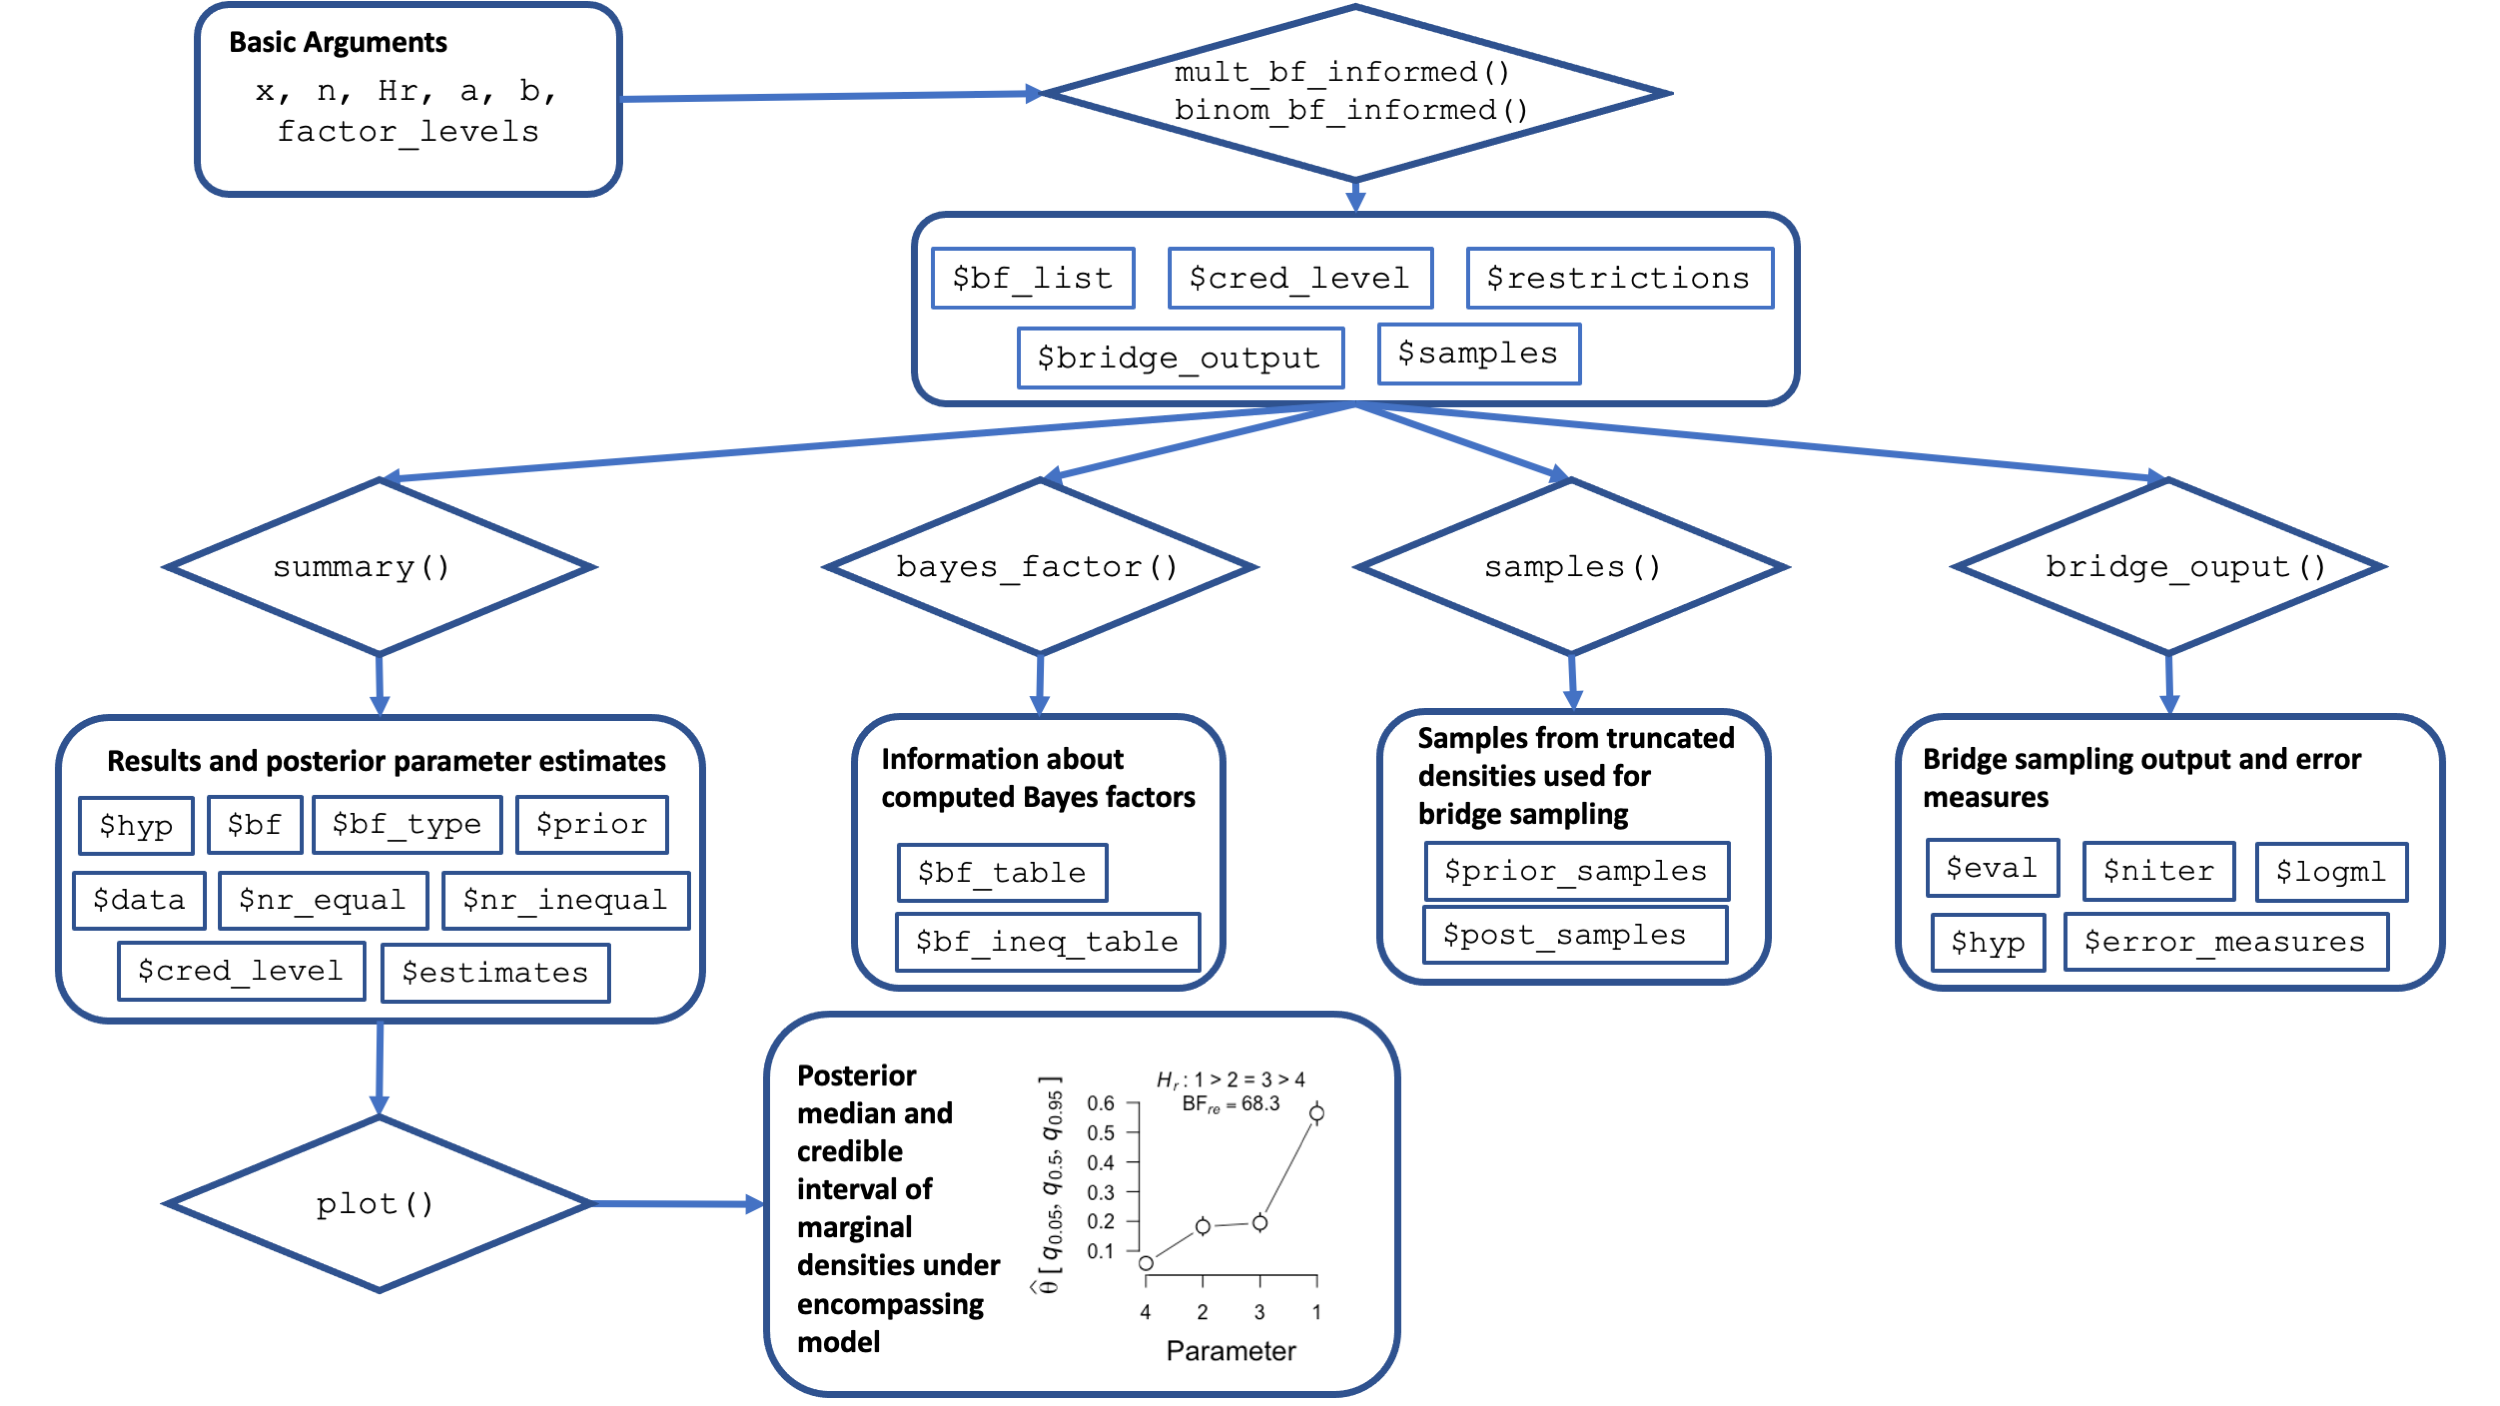
\includegraphics[width=400px]{scheme_multibridge} \caption{The \textbf{multibridge} workflow. When calling \texttt{mult\_bf\_informed} or \texttt{binom\_bf\_informed}, the user specifies the data values (\texttt{x} and \texttt{n} for binomial models and \texttt{x} for multinomial models, respectively), the informed hypothesis (\texttt{Hr}), the \(\alpha\) and \(\beta\) parameters of the binomial prior distributions (\texttt{a} and \texttt{b}) or the concentration parameters for the Dirichlet prior distribution (\texttt{a}), respectively, and the category labels of the factor levels (\texttt{factor\_levels}). The functions then return the estimated Bayes factor for the informed hypothesis relative to the encompassing or the null hypothesis. Based on these results different S3 methods can be used to get more detailed information on the individual components of the analysis (e.g., \texttt{summary}, \texttt{bayes\_factor}), and parameter estimates of the encompassing distribution (\texttt{plot}).}\label{fig:scheme-multibridge}
\end{figure}
\clearpage

\begin{table}[H]
\caption{To estimate the Bayes factor in favor for or against the specified informed hypothesis, the user provides the core functions \texttt{mult\_bf\_informed} and \texttt{binom\_bf\_informed} with the following basic required arguments listed below.}
\label{table:arguments}
\begin{center}
\begin{tabular}{p{4cm}p{12cm}}
        \toprule
Argument & Description \\\midrule
\texttt{x} & \texttt{numeric}. Vector with data (for multinomial models) or a vector of counts of successes, or a two-dimensional table (or matrix) with 2 columns, giving the counts of successes and failures, respectively (for binomial models).  \\
\texttt{n} &  \texttt{numeric}. Vector with counts of trials. Must be the same length as \texttt{x}. Ignored if \texttt{x} is a matrix or a table. Included only in \texttt{binom\_bf\_informed}. \\
\texttt{Hr} & \texttt{string} or \texttt{character}. String or vector with the user specified informed hypothesis. Users can either use the specified \texttt{factor\_levels} or numerical indices to refer to parameters.\\
\texttt{a} & \texttt{numeric}. Vector with concentration parameters of Dirichlet distribution (for multinomial models) or $\alpha$ parameters for independent beta distributions (for binomial models). Must be the same length as \texttt{x}. Default sets all parameters to 1. \\
\texttt{b} & \texttt{numeric}. Vector with $\beta$ parameters. Must be the same length as \texttt{x}. Default sets all $\beta$ parameters to 1. Included only in \texttt{binom\_bf\_informed}.\\
\texttt{factor\_levels} &  \texttt{character}. Vector with category labels. Must be the same length as \texttt{x}.\\
\bottomrule
\end{tabular}
\end{center}
\end{table}

\begin{table}[H]
\caption {S3 methods available in $\textbf{multibridge}$.}
\label{table:s3_methods}
\begin{center}
\begin{tabular}{p{4cm}p{3.5cm}p{9cm}}
        \toprule
Function Name(s) & S3 Method & Description \\\midrule
$\texttt{mult\_bf\_informed}$, $\texttt{binom\_bf\_informed}$ & $\texttt{print}$ & Prints model specifications and descriptives. \\
 & $\texttt{summary}$ &  Prints and returns the Bayes factor and associated hypotheses for the full model, and all equality and inequality constraints.\\
  & $\texttt{plot}$ &  Plots the posterior median and credible interval of the parameter estimates of the encompassing model. Default sets credible interval to 95\%.\\
 & $\texttt{bayes\_factor}$ & Contains all Bayes factors and log marginal likelihood estimates for inequality constraints.\\
 & $\texttt{samples}$ & Extracts prior and posterior samples from constrained densities (if bridge sampling was applied). \\
& $\texttt{bridge\_output}$    &  Extracts bridge sampling output and associated error measures.\\
& $\texttt{restriction\_list}$ & Extracts restriction list and associated informed hypothesis. \\
$\texttt{mult\_bf\_inequality}$, $\texttt{binom\_bf\_inequality}$  & $\texttt{print}$ & Prints the bridge sampling estimate for the log marginal likelihood and the corresponding percentage error. \\
& $\texttt{summary}$ & Prints and returns the bridge sampling estimate for the log marginal likelihood and associated error terms.\\
\bottomrule
\end{tabular}
\end{center}
\end{table}

\noindent This paper showcases how the proposed bridge sampling routine by Sarafoglou et al. (2020) can be applied in a user-friendly way with \textbf{multibridge}. In the remainder of this article, we will describe the Bayes factor identity for informed hypotheses in binomial and multinomial models, and briefly describe the bridge sampling method. Then, we illustrate the core functions of \textbf{multibridge} package using two examples and end with a brief summary.

\hypertarget{methods}{%
\section{Methods}\label{methods}}

\noindent In this section we formalize multinomial models and models that feature independent binomial probabilities as they have been implemented in \textbf{multibridge}. In the multinomial model, we assume that the vector of observations \textbf{x} in the \(K\) categories follows a multinomial distribution in which the parameters of interest, \(\boldsymbol{\theta}\), represent the underlying category proportions. Since the \(K\) categories are dependent, the vector of probability parameters is constrained to sum to one, such that \(\sum_{k = 1}^K (\theta_1, \cdots, \theta_K) = 1\). Therefore, a suitable choice for a prior distribution for \(\boldsymbol{\theta}\) is the Dirichlet distribution with concentration parameter vector \(\boldsymbol{\alpha}\):

\begin{align}
  x_1, \cdots, x_K &\sim \text{Multinomial}(\sum_{k = 1}^K x_k, \theta_1, \cdots, \theta_K) \\
  \theta_1, \cdots, \theta_K &\sim \text{Dirichlet}(\alpha_1, \cdots, \alpha_K),
\end{align}
where \(\boldsymbol{\alpha}\) can be interpreted as vector of \emph{a priori} category counts. The formalization of the model for independent binomial probabilities is very similar since the multinomial model above constitutes a generalization of the binomial model (for \(K \geq 2\)). In the binomial model, we assume that the elements in the vector of successes \textbf{x} and the elements in the vector of total number of observations \textbf{n} in the \(K\) categories follow independent binomial distributions. As in the multinomial model, the parameter vector of the binomial success probabilities \(\boldsymbol{\theta}\) contains the underlying category proportions, however, in this model we assume that categories are independent which removes the sum-to-one constraint. Therefore, a suitable choice for a prior distribution for \(\boldsymbol{\theta}\) is a vector of independent beta distributions with parameters \(\boldsymbol{\alpha}\) and \(\boldsymbol{\beta}\):

\begin{align}
  x_1 \cdots x_K & \sim \prod_{k = 1}^K \text{Binomial}(\theta_k, n_k) \\
  \theta_1 \cdots \theta_K &\sim \prod_{k = 1}^K \text{Beta}(\alpha_k, \beta_k),
\end{align}
where \(\boldsymbol{\alpha}\) can be interpreted as vector of \emph{a priori} successes that observations fall within the various categories and \(\boldsymbol{\beta}\) can be interpreted as vector of \emph{a priori} failures.

\hypertarget{bayes-factor}{%
\subsection{Bayes factor}\label{bayes-factor}}

\noindent In \textbf{multibridge} we use two different methods to compute Bayes factors: one method computes Bayes factors for equality constrained parameters and one method computes Bayes factors for inequality constrained parameters. Both methods will be outlined below. In cases where informed hypotheses feature mixtures between inequality and equality constraints, we compute the overall Bayes factor \(\text{BF}_{re}\) by multiplying the individual Bayes factors for both constraint types with each other. That is, the Bayes factor for mixtures factors into a Bayes factor for the equality constraints, and a conditional Bayes factor for the inequality constraints given the equality constraints (for the proof, see Sarafoglou et al., 2020).

\hypertarget{the-bayes-factor-for-equality-constraints}{%
\subsubsection{The Bayes Factor For Equality Constraints}\label{the-bayes-factor-for-equality-constraints}}

\noindent In \textbf{multibridge} the Bayes factor for the equality constraints can be computed analytically both for binomial and multinomial models using the functions \texttt{binom\_bf\_equality} and \texttt{mult\_bf\_equality}. For binomial models, assuming that the all binomial probabilities in a model are exactly equal, the Bayes factor is defined as:
\begin{align*}
\text{BF}_{0e}
&= \cfrac{\prod_{k=1}^K \text{B}(\alpha_k \text{, } \beta_k)}{\prod_{k=1}^K \text{B}(\alpha_k + x_k\text{, } \beta_k + n_k - x_k)} \times \cfrac{\text{B}(\alpha_+ + x_+ + 1\text{, } \beta_+ + n_+ - x_+ + 1)}{\text{B}(\alpha_+ + 1\text{, }\beta_+ + 1)},
\end{align*}
where \(\text{B}(\cdot)\) denotes the beta function and \(\alpha_+ = \sum_{k=1}^K\alpha_k\), \(\beta_+ = \sum_{k=1}^K\beta_k\), \(x_+ = \sum_{k=1}^K x_k\) and \(n_+ = \sum_{k=1}^K n_k\). If all binomial probabilities in a model are assumed to be exactly equal \textit{and} equal to a predicted value \(\theta_{0}\), the Bayes factor is defined as:
\begin{align*}
\text{BF}_{0e}
&= \cfrac{\prod_{k=1}^K \text{B}(\alpha_k \text{, } \beta_k)}{\prod_{k=1}^K \text{B}(\alpha_k + x_k\text{, } \beta_k + n_k - x_k)} \times \theta_{0}^{x_+} (1 - \theta_{0})^{n_+ - x_+}.
\end{align*}
Note that \textbf{multibridge} only supports the specification of one predicted value for all binomial probabilities. The package does not support the specification of different predicted values for different binomial probabilities. The reason for this is theoretical: we believe that such hypotheses are better tested using a hierarchical structure (thus modeling the binomial probabilities as dependent).

For multinomial models, assuming that all category probabilities in a model are equality constraint, the Bayes factor \(\text{BF}_{0e}\) is defined as:
\begin{align*}
\text{BF}_{0e} =  \frac{
 \text{B}\left(\alpha_{1}\text{, }\dots\text{, }\alpha_K\right)}{\text{B}\left(\alpha_1+x_1\text{, }\dots\text{, }\alpha_K+x_K\right)} \, \times 
\frac{\text{B}(\boldsymbol{\alpha}+\mathbf{x})}{\text{B}(\boldsymbol{\alpha})} \, \times  \prod_{k=1}^K \theta_{0k}^{x_k},
\end{align*}
where \(\theta_{0k}\) represent the predicted category proportions. When all category proportions are assumed to be exactly equal all \(\theta_{0k}\) are set to \(\frac{1}{K}\). Otherwise, \(\boldsymbol{\theta}_{0}\) is replaced with the user-specified predicted values.

\hypertarget{the-bayes-factor-for-inequality-constraints}{%
\subsubsection{The Bayes Factor For Inequality Constraints}\label{the-bayes-factor-for-inequality-constraints}}

\noindent To approximate the Bayes factor for informed hypotheses, Klugkist et al. (2005) derived an identity that defines the Bayes factor \(\text{BF}_{re}\) as ratio of proportions of posterior and prior parameter space consistent with the restriction. This identity forms the basis of the encompassing prior approach. Recently, Sarafoglou et al. (2020) highlighted that these proportions can be reinterpreted as the marginal likelihoods of the constrained posterior and constrained prior distribution:

\begin{align}
\label{Eq:klugkistIdentity}
\text{BF}_{re} &= \cfrac{\overbrace{p(\boldsymbol{\theta} \in \mathcal{R}_r \mid \mathbf{x}\text{, }\mathcal{H}_e)}^{\substack{\text{Marginal likelihood of}\\\text{constrained posterior distribution}}}}{\underbrace{p(\boldsymbol{\theta} \in \mathcal{R}_r \mid  \mathcal{H}_e)}_{\substack{\text{Marginal likelihood of}\\\text{constrained prior distribution}}}}.
\end{align}
The benefit of reinterpreting the identity by Klugkist et al. (2005) is that we can estimate the Bayes factor by utilizing numerical sampling methods such as bridge sampling. For that we only need to be able to sample from the constrained densities. Crucially, when using bridge sampling, it does not matter how small the constrained parameter space is in proportion to the encompassing density. This gives the method a decisive advantage over the encompassing prior approach in terms of accuracy and efficiency especially (1) when binomial and multinomial models with moderate to high number of categories (i.e., \(K > 10\)) are evaluated and (2) when relatively little posterior mass falls in the constrained parameter space.

The bridge sampling algorithm implemented in \textbf{multibridge} estimates one marginal likelihood at the time (cf., Gronau et al., 2017; Overstall \& Forster, 2010). Specifically, we subsequently estimate the marginal likelihood for the constrained prior distribution and the marginal likelihood of the constrained posterior distribution. Here we describe how to estimate the marginal likelihood for the constrained prior distribution, the steps presented can then be applied accordingly to the posterior distribution. It should be noted that the bridge sampling algorithm implemented in \textbf{multibridge}, is an adapted version of the algorithm implemented in the \texttt{R} package \textbf{bridgesampling} (Gronau, Singmann, \& Wagenmakers, 2020) and allows for the specification of informed hypotheses on probability vectors.\footnote{In addition, the function to compute the relative mean square error for bridge sampling estimates in \textbf{multibridge} is based on the code of the \texttt{error\_measures}-function from the \textbf{bridgesampling} package.} The bridge sampling identity for the marginal likelihood of the constrained prior distribution is defined as:

\begin{align}
    p(\boldsymbol{\theta} \in \mathcal{R}_r \mid \mathcal{H}_e) = \cfrac{\mathbb{E}_{g(\boldsymbol{\theta})}\left(p(\boldsymbol{\theta}\mid \mathcal{H}_e) \mathbb{I}(\boldsymbol{\theta}\in\mathcal{R}_r)h(\boldsymbol{\theta})\right)}{\mathbb{E}_{\text{prior}} \left(g(\boldsymbol{\theta})h(\boldsymbol{\theta})\right)},
    \label{Eq:bridgeidentity}
\end{align}
where the term \(h(\boldsymbol{\theta})\) refers to the bridge function proposed by Meng and Wong (1996), \(g(\boldsymbol{\theta})\) refers to a so-called proposal distribution, and \(p(\boldsymbol{\theta}\mid \mathcal{H}_e) \mathbb{I}(\boldsymbol{\theta}\in\mathcal{R}_r)\) is the part of the prior parameter space under the encompassing hypothesis that is in accordance with the constraint. To estimate the marginal likelihood, bridge sampling requires samples from the target distribution, that is, the constrained Dirichlet distribution for multinomial models and constrained beta distributions for binomial models, and samples from the proposal distribution which in principle can be any distribution with a known marginal likelihood; in \textbf{multibridge} the proposal distribution is the multivariate normal distribution. Samples from the target distribution are generated using the Gibbs sampling algorithms proposed by Damien and Walker (2001). For binomial models, we apply the suggested Gibbs sampling algorithm for constrained beta distributions. In the case of the multinomial models, we apply an algorithm that simulates values from constrained Gamma distributions which are then transformed into Dirichlet random variables. To sample efficiently from these distributions, \textbf{multibridge} provides a \texttt{C++} implementation of this algorithm. Samples from the proposal distribution are generated using the standard \texttt{rmvnorm}-function from the \texttt{R} package \textbf{mvtnorm} (Genz et al., 2020).

The efficiency of the bridge sampling method is optimal only if the target and proposal distribution operate on the same parameter space and have sufficient overlap. We therefore probit transform the samples of the constrained distributions to move the samples from the probability space to the entire real line. Subsequently, we use half of these draws to construct the proposal distribution using the method of moments. Details on the probit transformations are provided in the appendix.

The numerator in Equation \ref{Eq:bridgeidentity} evaluates the unnormalized density for the constrained prior distribution with samples from the proposal distribution. The denominator evaluates the normalized proposal distribution with samples from the constrained prior distribution. Using this identity, we receive the bridge sampling estimator for the marginal likelihood of the constrained prior distribution by applying the iterative scheme proposed by Meng and Wong (1996):

\begin{align*}
    \hat p(\boldsymbol{\theta} \in \mathcal{R}_r \mid \mathcal{H}_e)^{(t+1)} \approx \cfrac{\cfrac{1}{N_2} \sum_{m = 1}^{N_2} \cfrac{\ell_{2,m}}{s_1 \ell_{2,m} + s_2 p(\boldsymbol{\tilde \theta_m} \in \mathcal{R}_r \mid \mathcal{H}_e)^{(t)}}}
    {\cfrac{1}{N_1} \sum_{n = 1}^{N_1} \cfrac{1}{s_1 \ell_{1,n} + s_2 p(\boldsymbol{\theta^*_n} \in \mathcal{R}_r \mid \mathcal{H}_e)^{(t)}}},
    %\label{Eq:bridgeIterativeScheme}
\end{align*}
where \(N_1\) denotes the number of samples drawn from the constrained distribution, that is, \(\boldsymbol{\theta}^* \sim p(\boldsymbol{\theta} \mid \mathcal{H}_r)\), \(N_2\) denotes the number of samples drawn from the proposal distribution, that is \(\boldsymbol{\tilde \theta} \sim g(\boldsymbol{\theta})\),
\(s_1 = \frac{N_1}{N_2 + N_1}\), and \(s_2 = \frac{N_2}{N_2 + N_1}\). The quantities \(\ell_{1,n}\) and \(\ell_{2,m}\) are defined as follows:

\begin{align}
    \ell_{1,n} &= \cfrac{q_{1,1}}{q_{1,2}}  = \cfrac{p(\boldsymbol{\theta^*_n}\mid \mathcal{H}_e) \mathbb{I}(\boldsymbol{\theta^*_n}\in\mathcal{R}_r)}{g(\boldsymbol{\xi_n}^*)},\\
    \ell_{2,m} &= \cfrac{q_{2,1}}{q_{2,2}} = \cfrac{p(\boldsymbol{\tilde \theta_m}\mid \mathcal{H}_e) \mathbb{I}(\boldsymbol{\tilde \theta_m}\in\mathcal{R}_r)}{g(\boldsymbol{\tilde \xi_m})},
\end{align}
where \(\boldsymbol{\xi_n}^* = \Phi^{-1}\left(\cfrac{\boldsymbol{\theta^*_n} - \mathbf{l}}{\mathbf{u} - \mathbf{l}}\right)\), and \(\boldsymbol{\tilde \theta_m} = ((\mathbf{u} - \mathbf{l})\Phi(\boldsymbol{\tilde \xi_m}) + \mathbf{l}) \left|J\right|)\). The quantity \(q_{1,1}\) refers to the evaluations of the constrained distribution for constrained samples and \(q_{1,2}\) refers to the proposal distribution evaluated at the probit-transformed samples from the constrained distribution, respectively. The quantity \(q_{2,1}\) refers to evaluations of the constrained distribution at the inverse probit-transformed samples from the proposal distribution and \(q_{2,2}\) refers to the proposal evaluations for samples from the proposal, respectively. Note that the quantities \(\ell_{1,n}\) and \(\ell_{2,m}\) have been adjusted to account for the necessary parameter transformations to create overlap between the constrained distributions and the proposal distribution. \textbf{multibridge} runs the iterative scheme until the tolerance criterion suggested by Gronau et al. (2017) is reached, that is:
\begin{align*}
\cfrac{\mid \hat p(\boldsymbol{\theta} \in \mathcal{R}_r \mid \mathcal{H}_e)^{(t + 1)} - \hat p(\boldsymbol{\theta} \in \mathcal{R}_r \mid \mathcal{H}_e)^{(t)} \mid}{\hat p(\boldsymbol{\theta} \in \mathcal{R}_r \mid \mathcal{H}_e)^{(t + 1)}} &\leq 10^{-10}.
\end{align*}
The sampling from the target and proposal distribution, the transformations and computational steps are performed automatically within the core functions of \textbf{multibridge}. The user only needs to provide the functions with the data, a prior and a specification of the informed hypothesis. As part of the standard output of \texttt{binom\_bf\_informed} and \texttt{mult\_bf\_informed}, the functions return the bridge sampling estimate for the log marginal likelihood of the target distribution, its associate relative mean square error, the number of iterations, and the quantities \(q_{1,1}\), \(q_{1,2}\), \(q_{2,1}\), and \(q_{2,2}\).

\hypertarget{usage-and-examples}{%
\section{Usage and Examples}\label{usage-and-examples}}

\noindent In the following, we will outline two examples on how to use \textbf{multibridge} to compare an informed hypothesis to a null or encompassing hypothesis. In addition, the first example shows how two informed hypotheses can be compared to each other.

A list of all currently available functions and data sets is given in Table \ref{table:core_functions}. Additional examples are available as vignettes (see \url{https://cran.r-project.org/package=multibridge}, or \texttt{vignette(package\ =\ "multibridge")}). The two core functions of \textbf{multibridge}---\texttt{mult\_bf\_informed} and the \texttt{binom\_bf\_informed}---can be illustrated schematically as follows:

\begin{Shaded}
\begin{Highlighting}[]
\KeywordTok{mult_bf_informed}\NormalTok{(x, Hr, a, factor_levels)}
\KeywordTok{binom_bf_informed}\NormalTok{(x, n, Hr, a, b, factor_levels)}
\end{Highlighting}
\end{Shaded}

\begin{table}[H]
\caption {Core functions available in $\textbf{multibridge}$.}
\label{table:core_functions}
\begin{center}
\begin{tabular}{p{5.5cm}p{10.5cm}}
        \toprule
Function Name(s) & Description \\\midrule
$\texttt{mult\_bf\_informed}$ & Evaluates informed hypotheses on multinomial parameters.  \\
$\texttt{mult\_bf\_inequality}$ & Estimates the marginal likelihood of a constrained prior or posterior Dirichlet distribution.  \\
$\texttt{mult\_bf\_equality}$ & Computes Bayes factor for equality constrained multinomial parameters using the standard Bayesian multinomial test.  \\
$\texttt{mult\_tsampling}$ & Samples from constrained prior or posterior Dirichlet density.\\
$ \texttt{lifestresses}, \texttt{peas}$ & Data sets associated with informed hypotheses in multinomial models.\\\midrule
$\texttt{binom\_bf\_informed}$ & Evaluates informed hypotheses on binomial parameters.  \\
$\texttt{binom\_bf\_inequality}$ & Estimates the marginal likelihood of constrained prior or posterior beta distributions.\\
$\texttt{binom\_bf\_equality}$ & Computes Bayes factor for equality constrained binomial parameters.  \\
$\texttt{binom\_tsampling}$ & Samples from constrained prior or posterior beta densities.\\
$ \texttt{journals}$ & Data set associated with informed hypotheses in binomial models.\\\midrule
$ \texttt{generate\_restriction\_list}$ & Encodes the informed hypothesis.\\
\bottomrule
\end{tabular}
\end{center}
\end{table}

\hypertarget{example-1-applying-a-benford-test-to-greek-fiscal-data}{%
\subsection{Example 1: Applying A Benford Test to Greek Fiscal Data}\label{example-1-applying-a-benford-test-to-greek-fiscal-data}}

\noindent The first digit phenomenon, otherwise known as Benford's law (Benford, 1938; Newcomb, 1881) states that the expected proportion of leading digits in empirical data can be formalized as follows: for any given leading digit \(d, d = (1, \cdots, 9)\) the expected proportion is approximately equal to \[\mathbb{E}_{\theta_d}= \text{log}_{10}((d + 1)/d).\] This means that in an empirical data set numbers with smaller leading digits are more common than numbers with larger leading digits. Specifically, a number has leading digit \(1\) in \(30.1 \%\) of the cases, and leading digit \(2\) in \(17.61 \%\) of the cases; leading digit \(9\) is the least frequent digit with an expected proportion of only \(4.58 \%\) (see Table \ref{Tab:benford} for an overview of the expected proportions). Empirical data for which this relationship holds include population sizes, death rates, baseball statistics, atomic weights of elements, and physical constants (Benford, 1938). In contrast, generated data, such as telephone numbers, do in general not obey Benford's law (Hill, 1995). Given that Benford's law applies to empirical data but not artificially generated data, a so-called Benford test can be used in fields like accounting and auditing to check for indications for poor data quality (for an overview, see e.g., Durtschi, Hillison, \& Pacini, 2004; Nigrini, 2012; Nigrini \& Mittermaier, 1997). Data that do not pass the Benford test, should raise audit risk concerns, meaning that it is recommended that they undergo additional follow-up checks (Nigrini, 2019).

Below, we discuss three possible Bayesian adaptations of the Benford's test. In a first scenario we simply conduct a Bayesian multinomial test in which we test the point-null hypothesis \(\mathcal{H}_0\) which predicts a Benford distribution against the encompassing hypothesis \(\mathcal{H}_{e}\). In a second scenario we test the null hypothesis against an alternative hypothesis, denoted as \(\mathcal{H}_{r1}\), which predicts a decreasing trend in the proportions of leading digits. The hypothesis \(\mathcal{H}_{r1}\) exerts considerably more constraints than \(\mathcal{H}_{e}\) and provides a more sensitive test if our primary goal is to test whether data comply with Benford's law or whether the data follow a similar but different trend. In a third scenario, where the main goal is to identify fabricated data, we test the null hypothesis against a hypothesis which predicts a trend that is characteristic for manipulated data. This hypothesis, which we denote as \(\mathcal{H}_{r2}\), could be derived from empirical research on fraud or be based on observed patterns from former fraud cases. For instance, Hill (1988) instructed students to produce a series of random numbers; in the resulting data the proportion of the leading digit \(1\) occurred most often and the digits \(8\) and \(9\) occurred least often which is consistent with the general pattern of Benford's law. However, the proportion for the remaining leading digits were approximately equal. Note that the predicted distribution derived from Hill (1988) is not currently used as a test to detect fraud. However, for the sake of simplicity, if we assume that this pattern could be an indication of fabricated auditing data, the Bayes factor would quantify the evidence of whether the proportion of first digits resemble authentic or fabricated data.

\hypertarget{data-and-hypothesis}{%
\subsubsection{Data and Hypothesis}\label{data-and-hypothesis}}

The data we use to illustrate the computation of Bayes factors were originally published by the European statistics agency \enquote{Eurostat} and served as basis for reviewing the adherence to the Stability and Growth Pact of EU member states. Rauch, Göttsche, Brähler, and Engel (2011) conducted a Benford test on data related to budget deficit criteria, that is, public deficit, public dept and gross national products. The data used for this example features the proportion of first digits from fiscal data from Greece in the years between \(1999\) and \(2010\); a total of \(N= 1{,}497\) numerical data were included in the analysis. We choose this data, since the Greek government deficit and debt statistics states has been repeatedly criticized by the European Commission in this time span (European Commision, 2004, 2010). In particular, the commission has accused the Greek statistical authorities to have misreported deficit and debt statistics. For further details on the data set see Rauch et al. (2011). The observed proportions are displayed in Table \ref{Tab:benford}, the figure displaying the observed versus the expected proportions are displayed in Figure \ref{fig:benford-alt}.

\begin{table}[H]
    \centering
    \caption{The Table shows the Observed Counts, Observed Proportions, and Expected Proportions of first digits in Greece governmental data. The total sample size was $N = 1{,}497$ observations. Note that the observed proportions and counts deviate slightly from those reported in Rauch et al. (2011) (probably due to rounding errors).}
    \begin{tabular}{cccp{4cm}}
        \hline
Leading digit & Observed Counts & Observed Proportions & Expected Proportions: Benford's Law  \\
        \hline
        1 & 509 & 0.340 & 0.301  \\
        2 & 353 & 0.236 & 0.176  \\
        3 & 177 & 0.118 & 0.125  \\
        4 & 114 & 0.076 & 0.097  \\
        5 & 77 & 0.051 & 0.079  \\
        6 & 77 & 0.051 & 0.067  \\
        7 & 53 & 0.035 & 0.058  \\
        8 & 73 & 0.049 & 0.051  \\
        9 & 64 & 0.043 & 0.046  \\
        \hline
    \end{tabular}
    \label{Tab:benford}
\end{table}

In this example, the parameter vector of the multinomial model, \(\theta_1, \cdots, \theta_K\), reflects the probabilities of a leading digit in the Greek fiscal data being a number from \(1\) to \(9\). Thus, we can formalize the discussed hypotheses as follows. The null hypothesis specifies that the proportions of first digits obeys Benford's law:
\[\mathcal{H}_0 : \boldsymbol{\theta}_0 = (0.301, 0.176, 0.125, 0.097, 0.079, 0.067, 0.058, 0.051, 0.046).\]

Here, we are testing the null hypothesis against the following three alternative hypotheses:
\begin{align*}
\mathcal{H}_e &: \boldsymbol{\theta} \sim \text{Dirichlet}(\boldsymbol{\alpha}), \\
\mathcal{H}_{r1} &: \theta_1 > \theta_2 > \theta_3 > \theta_4 > \theta_5 > \theta_6 > \theta_7 > \theta_8 > \theta_9, \\
\mathcal{H}_{r2} &:  \theta_1 > (\theta_2 = \theta_3 = \theta_4 = \theta_5 = \theta_6 = \theta_7) > (\theta_8, \ \theta_9).
\end{align*}

We could also compare the three alternative hypothesis directly with each other. To do so, we can make use of the transitivity property of the Bayes factor. For instance, if we would like to compare \(\mathcal{H}_{r1}\) with \(\mathcal{H}_{r2}\), we would first compute \(\text{BF}_{er1}\) and \(\text{BF}_{er2}\) and then yield \(\text{BF}_{r1r2}\) by dividing the two quantities:
\[\text{BF}_{r1r2} = \cfrac{\text{BF}_{er2}}{\text{BF}_{er1}}.\]

\hypertarget{method}{%
\subsubsection{Method}\label{method}}

We can compare \(\mathcal{H}_0\) and \(\mathcal{H}_e\) by means of a Bayesian multinomial test which is implemented in the function \texttt{mult\_bf\_equality}. To evaluate \(\mathcal{H}_0\), we only need to specify (1) a vector with observed counts, (2) a vector with concentration parameters of the Dirichlet prior distribution, and (3) the vector of proportions expected under the null hypothesis. We do not want to incorporate any specific expectations about the distribution of leading digits in the Greek fiscal data. Hence, we set all concentration parameters to one which corresponds to a uniform Dirichlet distribution.

\begin{Shaded}
\begin{Highlighting}[]
\CommentTok{# Observed counts}
\NormalTok{x <-}\StringTok{ }\KeywordTok{c}\NormalTok{(}\DecValTok{509}\NormalTok{, }\DecValTok{353}\NormalTok{, }\DecValTok{177}\NormalTok{, }\DecValTok{114}\NormalTok{,  }\DecValTok{77}\NormalTok{,  }\DecValTok{77}\NormalTok{,  }\DecValTok{53}\NormalTok{,  }\DecValTok{73}\NormalTok{,  }\DecValTok{64}\NormalTok{)}
\CommentTok{# Concentration parameters}
\NormalTok{a <-}\StringTok{  }\KeywordTok{rep}\NormalTok{(}\DecValTok{1}\NormalTok{, }\DecValTok{9}\NormalTok{)}
\CommentTok{# Expected proportions}
\NormalTok{p <-}\StringTok{ }\KeywordTok{log10}\NormalTok{((}\DecValTok{1}\OperatorTok{:}\DecValTok{9} \OperatorTok{+}\StringTok{ }\DecValTok{1}\NormalTok{)}\OperatorTok{/}\DecValTok{1}\OperatorTok{:}\DecValTok{9}\NormalTok{)}
\CommentTok{# Execute the analysis}
\NormalTok{results_H0_He  <-}\StringTok{ }\KeywordTok{mult_bf_equality}\NormalTok{(}\DataTypeTok{x =}\NormalTok{ x, }\DataTypeTok{a =}\NormalTok{ a, }\DataTypeTok{p =}\NormalTok{ p)}
\NormalTok{logBFe0 <-}\StringTok{ }\NormalTok{results_H0_He}\OperatorTok{$}\NormalTok{bf}\OperatorTok{$}\NormalTok{LogBFe0}
\end{Highlighting}
\end{Shaded}

Since the hypotheses \(\mathcal{H}_{r1}\) and \(\mathcal{H}_{r2}\) contain inequality constraints, we use the function \texttt{mult\_bf\_informed} to compute the Bayes factor of the informed hypotheses to the encompassing hypothesis. We then make use of the transitivity property of the Bayes factor to compare the alternative hypotheses to the null hypothesis. In this function, we need to specify (1) a vector with observed counts, (2) the informed hypothesis \(\mathcal{H}_{r1}\) or \(\mathcal{H}_{r2}\) (e.g., as character vector), (3) a vector with concentration parameters of the Dirichlet prior distribution, and (4) labels for the categories of interest (i.e., leading digits):

\begin{Shaded}
\begin{Highlighting}[]
\CommentTok{# Labels for categories of interest}
\NormalTok{factor_levels <-}\StringTok{ }\DecValTok{1}\OperatorTok{:}\DecValTok{9}
\CommentTok{# Specifying the informed Hypothesis}
\NormalTok{Hr1 <-}\StringTok{ }\KeywordTok{c}\NormalTok{(}\StringTok{'1 > 2 > 3 > 4 > 5 > 6 > 7 > 8 > 9'}\NormalTok{)}
\NormalTok{Hr2 <-}\StringTok{ }\KeywordTok{c}\NormalTok{(}\StringTok{'1 > 2 = 3 = 4 = 5 = 6 = 7 > 8 > 9'}\NormalTok{)}
\CommentTok{# Execute the analysis}
\NormalTok{results_He_Hr1 <-}\StringTok{ }\KeywordTok{mult_bf_informed}\NormalTok{(}\DataTypeTok{x =}\NormalTok{ x, }\DataTypeTok{Hr =}\NormalTok{ Hr1, }\DataTypeTok{a =}\NormalTok{ a, }
                                 \DataTypeTok{factor_levels =}\NormalTok{ factor_levels, }
                                 \DataTypeTok{bf_type =} \StringTok{'LogBFer'}\NormalTok{, }\DataTypeTok{seed =} \DecValTok{2020}\NormalTok{)}
\NormalTok{logBFer1 <-}\StringTok{ }\KeywordTok{summary}\NormalTok{(results_He_Hr1)}\OperatorTok{$}\NormalTok{bf}
\NormalTok{results_He_Hr2 <-}\StringTok{ }\KeywordTok{mult_bf_informed}\NormalTok{(}\DataTypeTok{x =}\NormalTok{ x, }\DataTypeTok{Hr =}\NormalTok{ Hr2, }\DataTypeTok{a =}\NormalTok{ a, }
                                 \DataTypeTok{factor_levels =}\NormalTok{ factor_levels, }
                                 \DataTypeTok{bf_type =} \StringTok{'LogBFer'}\NormalTok{, }\DataTypeTok{seed =} \DecValTok{2020}\NormalTok{)}
\NormalTok{logBFer2 <-}\StringTok{ }\KeywordTok{summary}\NormalTok{(results_He_Hr2)}\OperatorTok{$}\NormalTok{bf}
\end{Highlighting}
\end{Shaded}

\begin{Shaded}
\begin{Highlighting}[]
\NormalTok{bayes_factor_table <-}\StringTok{ }\KeywordTok{data.frame}\NormalTok{(}
   \DataTypeTok{BFType =} \KeywordTok{c}\NormalTok{(}\StringTok{'LogBFe0'}\NormalTok{, }\StringTok{'LogBFr10'}\NormalTok{, }\StringTok{'LogBFr20'}\NormalTok{), }
   \DataTypeTok{LogBF  =} \KeywordTok{c}\NormalTok{(logBFe0, }\OperatorTok{-}\NormalTok{logBFer1 }\OperatorTok{+}\StringTok{ }\NormalTok{logBFe0, }\OperatorTok{-}\NormalTok{logBFer2 }\OperatorTok{+}\StringTok{ }\NormalTok{logBFe0))}
\NormalTok{bayes_factor_table}
\end{Highlighting}
\end{Shaded}

\begin{verbatim}
##     BFType     LogBF
## 1  LogBFe0   17.6715
## 2 LogBFr10   25.0883
## 3 LogBFr20 -154.5685
\end{verbatim}

As the evidence is extreme in all three cases, we report all Bayes factors on the log scale. We can make the following statements concerning the comparison of the null hypothesis to the three alternative hypotheses. The first Bayes factor \(\text{log}(\text{BF}_{e0})\) suggests extreme evidence \textit{in favor of} the hypothesis that the first digits vary freely; \(\text{log}(\text{BF}_{e0}) =\) 17.67. The second Bayes factor \(\text{log}(\text{BF}_{r10})\) suggests extreme evidence \textit{in favor of} the hypothesis that the first digits follow a decreasing trend, \(\text{log}(\text{BF}_{r10}) =\) 25.09. The third Bayes factor \(\text{log}(\text{BF}_{r20})\) suggests extreme evidence \textit{against} the hypothesis that the first digits follow a fraudulent pattern with \(\text{log}(\text{BF}_{r20}) =\) -154.57. When we compare the informed hypotheses \(\mathcal{H}_{r1}\) and \(\mathcal{H}_{r2}\) directly with each other, the data show most evidence for a decreasing trend (\(\text{log}(\text{BF}_{r1r2}) =\) 180).



\begin{figure}
\centering
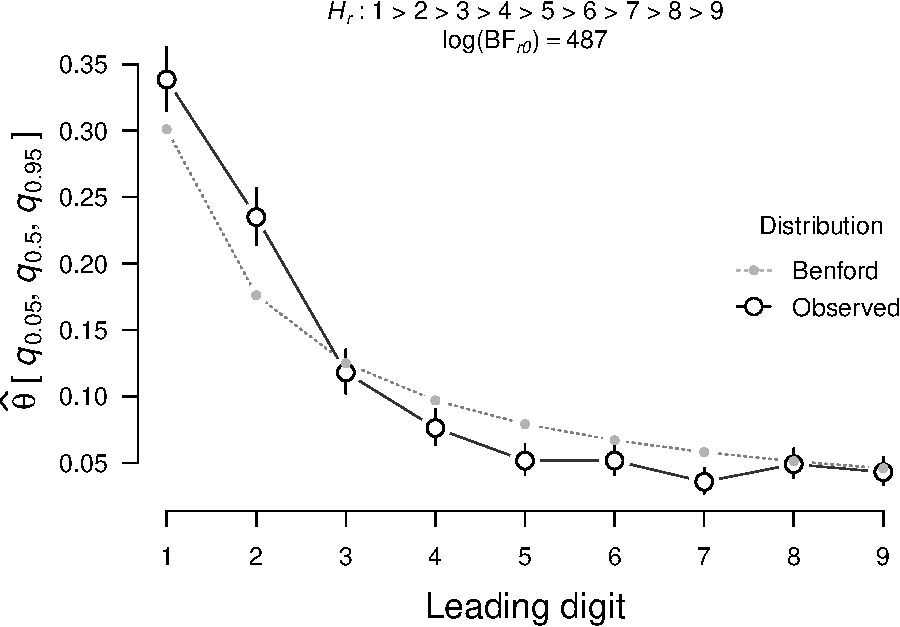
\includegraphics{Rpackage_paper_files/figure-latex/benford-alt-1.pdf}
\caption{\label{fig:benford-alt}Proportions of leading digits observed in the fiscal statistics from Greece in comparison to the proportions expected according to Benford's law. The black-rimmed dots indicate the the posterior median estimates and corresponding 95\% credible intervals based on the encompassing model. The grey filled dots indicate the proportions predicted by Benford's law. Only three out of nine estimates cover the expected proportions. This plot was created using the \texttt{plot}-S3-method for \texttt{summary.bmult} objects.}
\end{figure}

To summarize, the preferred hypothesis is \(\mathcal{H}_{r1}\) that postulates an decreasing trend. The second best performing hypothesis is the encompassing hypothesis \(\mathcal{H}_{e}\), followed by \(\mathcal{H}_{0}\) that postulates a Benford distribution. The worst performing hypothesis is \(\mathcal{H}_{r2}\), the hypothesis that the data are fabricated. Hence, the result suggests that the leading digits in the fiscal statistics do not follow a Benford distribution but they also do not seem to be fabricated. Therefore, it might be reasonable to assume that the data have poor overall quality. Further follow-up checks of these numbers could provide information on whether financial statements were actually materially misstated, for instance, by rounding up or down numbers, avoiding certain thresholds and so on (Nigrini, 2019).

\hypertarget{example-2-prevalence-of-statistical-reporting-errors}{%
\subsection{Example 2: Prevalence of Statistical Reporting Errors}\label{example-2-prevalence-of-statistical-reporting-errors}}

In any scientific article that uses null hypothesis significance testing, there is a chance that the reported test statistic and degrees of freedom do not match the reported \(p\)-value. In most cases this is because researchers copy the relevant test statistics by hand into their articles and there are no automatic checks to detect mistakes. Therefore, Epskamp and Nuijten (2014) developed the R package \texttt{statcheck}, which only requires the PDF of a given scientific article to detect these reporting errors automatically and efficiently. This package allowed Nuijten et al. (2016) to estimate the prevalence of statistical reporting errors in the field of psychology. In total, the authors investigated a sample of \(30{,}717\) articles (which translates to over a quarter of a million \(p\)-values) published in eight major psychological journals between 1985 to 2013: \emph{Developmental Psychology} (DP), the \emph{Frontiers in Psychology} (FP), the \emph{Journal of Applied Psychology} (JAP), the \emph{Journal of Consulting and Clinical Psychology} (JCCP), \emph{Journal of Experimental Psychology: General} (JEPG), the \emph{Journal of Personality and Social Psychology} (JPSP), the \emph{Public Library of Science} (PLoS), \emph{Psychological Science} (PS).

Besides the overall prevalence of statistical reporting errors across these journals, the authors were interested whether there is a higher prevalence for reporting inconsistencies in certain subfields in psychology compared to others. In this context, the possibility was raised that there exists a relationship between the prevalence for reporting inconsistencies and questionable research practices. Specifically, the authors argued that besides honest mistakes when transferring the test statistics into the manuscript, statistical reporting errors occur when authors misreport \(p\)-values, for instance, by incorrectly rounding them down to or below \(0.05\). Based on this assumption, Nuijten et al. (2016) predicted that the proportion of statistical reporting errors should be highest in articles published in the \emph{Journal of Personality and Social Psychology} (JPSP), compared to other journals, because compared to other areas of psychology researchers in social psychology most frequently deemed questionable research practices defensible and applicable to their research (John, Loewenstein, \& Prelec, 2012).

\hypertarget{data-and-hypothesis-1}{%
\subsubsection{Data and Hypothesis}\label{data-and-hypothesis-1}}

Here, we reuse the original data published by Nuijten et al. (2016), which we also distribute with the package \textbf{multibridge} under the name \texttt{journals}.

\begin{Shaded}
\begin{Highlighting}[]
\KeywordTok{data}\NormalTok{(journals)}
\end{Highlighting}
\end{Shaded}

The hypothesis of interest, \(\mathcal{H}_r\), formulated by Nuijten et al. (2016) states that the prevalence for statistical reporting errors for articles published in social psychology journals (i.e., JPSP) is higher than for articles published in other journals. Note that Nuijten et al. (2016) did not make use of inferential statistics since their sample included the entire population of articles from the eight flagship journals in psychology from 1985 to 2013. For demonstration purposes, however, we will test the informed hypothesis stated by the authors. We will test \(\mathcal{H}_r\) against the the null hypothesis \(\mathcal{H}_0\) that all journals have the same prevalence for statistical reporting errors. In this example, the parameter vector of the binomial success probabilities, \(\boldsymbol{\theta}\), reflects the probabilities that articles using null hypothesis significance testing (NHST) will have at least one statistical reporting error across journals. Thus, we can formalize the discussed hypotheses as follows:

\begin{align*}
    \mathcal{H}_r &: (\theta_{\text{DP}}, \theta_{\text{FP}}, \theta_{\text{JAP}} , \theta_{\text{JCCP}} , \theta_{\text{JEPG}} , \theta_{\text{PLoS}}, \theta_{\text{PS}}) < \theta_{\text{JPSP}} \\
    \mathcal{H}_0 &: \theta_{\text{DP}} =  \theta_{\text{FP}} =  \cdots = \theta_{\text{JPSP}}.
\end{align*}

\hypertarget{method-1}{%
\subsubsection{Method}\label{method-1}}

To compute the Bayes factor \(\text{BF}_{0r}\) we need to specify (1) a vector with observed successes (i.e., number of articles that contain a statistical reporting error), and (2) a vector containing the total number of observations, (3) the informed hypothesis, (4) a vector with prior parameter \(\alpha_i\) for each binomial proportion, (5) a vector with prior parameter \(\beta_i\) for each binomial proportion, and (6) the category labels (i.e., journal names). Since we have no specific expectations about the distribution of statistical reporting errors in any given journal, we set all parameters \(\alpha_i\) and \(\beta_i\) to one which corresponds to uniform beta distributions. With this information, we can now conduct the analysis with the function \texttt{binom\_bf\_informed}.

\begin{Shaded}
\begin{Highlighting}[]
\CommentTok{# Since percentages are rounded to two decimal values, we round the}
\CommentTok{# articles with an error to obtain integer values}
\NormalTok{x <-}\StringTok{ }\KeywordTok{round}\NormalTok{(journals}\OperatorTok{$}\NormalTok{articles_with_NHST  }\OperatorTok{*}\StringTok{ }
\StringTok{             }\NormalTok{(journals}\OperatorTok{$}\NormalTok{perc_articles_with_errors}\OperatorTok{/}\DecValTok{100}\NormalTok{))}

\CommentTok{# Total number of articles}
\NormalTok{n <-}\StringTok{ }\NormalTok{journals}\OperatorTok{$}\NormalTok{articles_with_NHST}

\CommentTok{# Prior specification}
\CommentTok{# We assign a uniform beta distribution to each binomial proportion}
\NormalTok{a <-}\StringTok{ }\KeywordTok{rep}\NormalTok{(}\DecValTok{1}\NormalTok{, }\DecValTok{8}\NormalTok{)}
\NormalTok{b <-}\StringTok{ }\KeywordTok{rep}\NormalTok{(}\DecValTok{1}\NormalTok{, }\DecValTok{8}\NormalTok{)}

\CommentTok{# Specifying the informed Hypothesis}
\NormalTok{Hr <-}\StringTok{ }\KeywordTok{c}\NormalTok{(}\StringTok{'JAP , PS , JCCP , PLOS , DP , FP , JEPG < JPSP'}\NormalTok{)}

\CommentTok{# Category labels}
\NormalTok{journal_names <-}\StringTok{ }\NormalTok{journals}\OperatorTok{$}\NormalTok{journal}

\CommentTok{# Execute the analysis}
\NormalTok{results_H0_Hr <-}\StringTok{ }\KeywordTok{binom_bf_informed}\NormalTok{(}\DataTypeTok{x =}\NormalTok{ x, }\DataTypeTok{n =}\NormalTok{ n, }\DataTypeTok{Hr =}\NormalTok{ Hr, }\DataTypeTok{a =}\NormalTok{ a, }\DataTypeTok{b =}\NormalTok{ b,}
                               \DataTypeTok{factor_levels =}\NormalTok{ journal_names,}
                               \DataTypeTok{bf_type =} \StringTok{'LogBFr0'}\NormalTok{, }\DataTypeTok{seed =} \DecValTok{2020}\NormalTok{)}
\end{Highlighting}
\end{Shaded}

\begin{Shaded}
\begin{Highlighting}[]
\NormalTok{LogBFr0 <-}\StringTok{ }\KeywordTok{summary}\NormalTok{(results_H0_Hr)}\OperatorTok{$}\NormalTok{bf}
\NormalTok{LogBFe0 <-}\StringTok{ }\NormalTok{results_H0_Hr}\OperatorTok{$}\NormalTok{bf_list}\OperatorTok{$}\NormalTok{bf0_table[[}\StringTok{'LogBFe0'}\NormalTok{]]}
\NormalTok{LogBFre <-}\StringTok{ }\OperatorTok{-}\NormalTok{results_H0_Hr}\OperatorTok{$}\NormalTok{bf_list}\OperatorTok{$}\NormalTok{bfr_table[[}\StringTok{'LogBFer'}\NormalTok{]]}

\NormalTok{bayes_factor_table <-}\StringTok{ }\KeywordTok{data.frame}\NormalTok{(}
   \DataTypeTok{BFType =} \KeywordTok{c}\NormalTok{(}\StringTok{'LogBFe0'}\NormalTok{, }\StringTok{'LogBFr0'}\NormalTok{, }\StringTok{'LogBFre'}\NormalTok{), }
   \DataTypeTok{BF =} \KeywordTok{c}\NormalTok{(LogBFe0, LogBFr0, LogBFre))}
\NormalTok{bayes_factor_table}
\end{Highlighting}
\end{Shaded}

\begin{verbatim}
##    BFType         BF
## 1 LogBFe0 156.272164
## 2 LogBFr0 158.280000
## 3 LogBFre   2.005374
\end{verbatim}

Again, as the evidence is extreme in all three cases, we report all Bayes factors on the log scale. The Bayes factor \(\log(\text{BF}_{r0})\) suggests extreme evidence for the informed hypothesis that the social psychology journal JPSP has the highest prevalence for statistical reporting errors compared to the null hypothesis that the statistical reporting errors are equal across journals; \(\log(\text{BF}_{r0}) = 158.28\).

In order to get a clearer picture about the ordering of the journals, we can investigate the posterior estimates
under the encompassing model as the next step. The posterior median and 95\% credible interval are returned by the \texttt{summary}-method and can be plotted, Figure~\ref{fig:journals}.



\begin{figure}
\centering
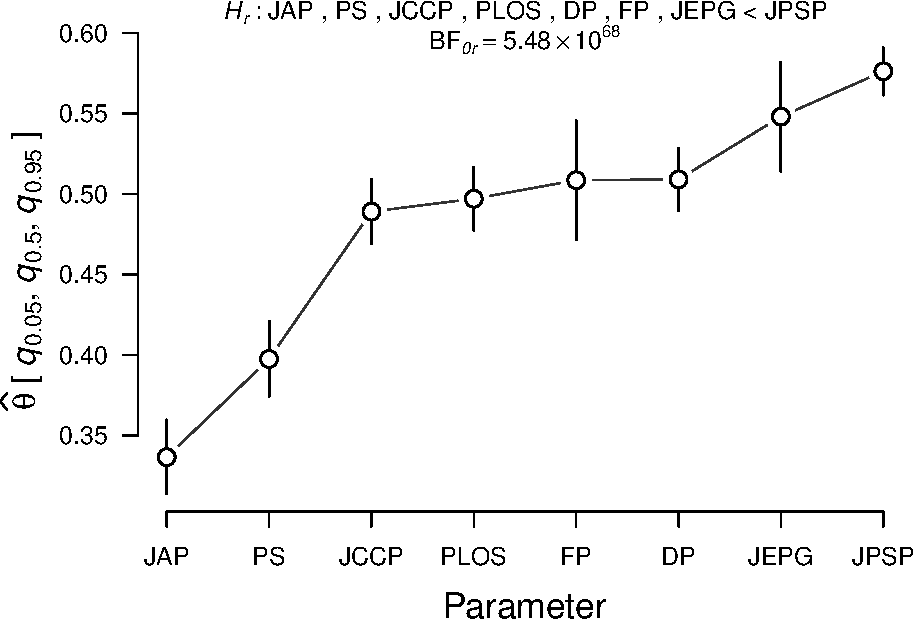
\includegraphics{Rpackage_paper_files/figure-latex/journals-1.pdf}
\caption{\label{fig:journals}The figure displays for each journal the posterior estimates for the prevalence that an article includes a statistical reporting error and the corresponding 95\% credible intervals based on the encompassing model. It appears that all journals show a relatively similar prevalence for statistical reporting errors, with the exception of the \emph{Journal of Applied Psychology} (JAP) and \emph{Psychological Science} (PS), whose prevalence is much lower. This plot was created using the \texttt{plot}-S3-method for \texttt{summary.bmult} objects.}
\end{figure}

When comparing \(\mathcal{H}_r\) and \(\mathcal{H}_0\) with the encompassing hypothesis, we also see that the data suggest that the null hypothesis that the statistical reporting errors are equal across journals is highly unlikely compared to the encompassing hypothesis, \(\log(\text{BF}_{e0}) = 156.27\). In addition, the results the data suggest moderate evidence for the informed hypothesis compared to the hypothesis that the ordering of the journals can vary freely, \(\log(\text{BF}_{re}) = 2.01\).

To summarize, we collected extreme evidence for the hypothesis stated by Nuijten et al. (2016) that the prevalence of statistical reporting errors for articles published in a social psychology journal (i.e., JPSP) is higher than for articles published in other journals. However, this result should be interpreted with caution. It seems that the result is above all an indication that the null hypothesis is highly misspecified and that the prevalence for a statistical reporting error varies greatly from journal to journal. Evidence that JPSP stands out and has a higher prevalence than the other journals is relatively small; the data provided only moderate evidence against the encompassing hypotheses.

\hypertarget{summary}{%
\section{Summary}\label{summary}}

The \texttt{R} package \textbf{multibridge} facilitates the estimation of Bayes factors for informed hypotheses in binomial and multinomial models. Compared to existing packages, this new package efficiently estimates Bayes factors for models with large number of categories which occur frequently in empirical studies. This efficient and reliable estimation is made possible by a recently developed bridge sampling routine (Sarafoglou et al., 2020). The package offers researchers and practitioners the opportunity to specify informed hypotheses that relate closely to their theories. Specifically, informed hypotheses that feature equality constraints, inequality constraints, and free parameters as well as mixtures between them are supported. Moreover, users can also choose whether the informative hypothesis should be tested against an encompassing hypothesis that lets all parameters vary freely or the null hypothesis that states that category proportions are exactly equal.

Beyond the core functions currently implemented in \textbf{multibridge}, there are several natural extensions we aim to include in future versions of this package. For instance, one extension is to facilitate the specification of hierarchical binomial and multinomial models which would allow users to analyze data where responses are nested within participants. Hierarchical multinomial models can be found, for instance, in source memory research where participants need to select a previously studied item from a list of multiple stimuli (e.g., Arnold, Heck, Bröder, Meiser, \& Boywitt, 2019). In addition, we aim to enable the specification of informed hypotheses that are more complex, including hypotheses on the size ratios of the parameters of interest or the difference between category proportions such that informed hypotheses can also be specified on odds ratios.

\hypertarget{acknowledgements}{%
\section{Acknowledgements}\label{acknowledgements}}

This research was supported by a Netherlands Organisation for Scientific Research (NWO) grant
to AS (406-17-568), a Veni grant from the NWO to MM (451-17-017), a Vici grant from the NWO to EJW (016.Vici.170.083), as well as a a European Research Council (ERC) grant to EJW (283876).

\clearpage

\hypertarget{references}{%
\section{References}\label{references}}

\begingroup
\setlength{\parindent}{-0.5in}
\setlength{\leftskip}{0.5in}

\hypertarget{refs}{}
\leavevmode\hypertarget{ref-arnold2019testing}{}%
Arnold, N. R., Heck, D. W., Bröder, A., Meiser, T., \& Boywitt, C. D. (2019). Testing hypotheses about binding in context memory with a hierarchical multinomial modeling approach. \emph{Experimental Psychology}, \emph{66}, 239--251.

\leavevmode\hypertarget{ref-benford1938law}{}%
Benford, F. (1938). The law of anomalous numbers. \emph{Proceedings of the American Philosophical Society}, 551--572.

\leavevmode\hypertarget{ref-bennett1976efficient}{}%
Bennett, C. H. (1976). Efficient estimation of free energy differences from Monte Carlo data. \emph{Journal of Computational Physics}, \emph{22}, 245--268.

\leavevmode\hypertarget{ref-damien2001sampling}{}%
Damien, P., \& Walker, S. G. (2001). Sampling truncated normal, beta, and gamma densities. \emph{Journal of Computational and Graphical Statistics}, \emph{10}, 206--215.

\leavevmode\hypertarget{ref-durtschi2004effective}{}%
Durtschi, C., Hillison, W., \& Pacini, C. (2004). The effective use of benford's law to assist in detecting fraud in accounting data. \emph{Journal of Forensic Accounting}, \emph{5}, 17--34.

\leavevmode\hypertarget{ref-epskamp2014statcheck}{}%
Epskamp, S., \& Nuijten, M. (2014). \emph{Statcheck: Extract statistics from articles and recompute p values (R package version 1.0.0.)}. Comprehensive R Archive Network. Retrieved from \url{https://cran.r-project.org/web/packages/statcheck}

\leavevmode\hypertarget{ref-europeanCommision2004}{}%
European Commision. (2004). \emph{Report by Eurostat on the revision of the Greek government deficit and debt figures} {[}Eurostat Report{]}. \url{https://ec.europa.eu/eurostat/web/products-eurostat-news/-/GREECE}.

\leavevmode\hypertarget{ref-europeanCommision2010}{}%
European Commision. (2010). \emph{Report on Greek government deficit and debt statistics} {[}Eurostat Report{]}. \url{https://ec.europa.eu/eurostat/web/products-eurostat-news/-/COM_2010_REPORT_GREEK}.

\leavevmode\hypertarget{ref-mvtnorm}{}%
Genz, A., Bretz, F., Miwa, T., Mi, X., Leisch, F., \& Hothorn, F. S. T. (2020). \emph{Mvtnorm: Multivariate normal and t distributions}. Retrieved from \url{http://CRAN.R-project.org/package=mvtnorm}

\leavevmode\hypertarget{ref-gronau2017tutorial}{}%
Gronau, Q. F., Sarafoglou, A., Matzke, D., Ly, A., Boehm, U., Marsman, M., \ldots{} Steingroever, H. (2017). A tutorial on bridge sampling. \emph{Journal of Mathematical Psychology}, \emph{81}, 80--97.

\leavevmode\hypertarget{ref-gronau2017bridgesampling}{}%
Gronau, Q. F., Singmann, H., \& Wagenmakers, E. (2020). Bridgesampling: An R package for estimating normalizing constants. \emph{Journal of Statistical Software, Articles}, \emph{92}(10), 1--29.

\leavevmode\hypertarget{ref-gu2019bain}{}%
Gu, X., Hoijtink, H., Mulder, J., \& Rosseel, Y. (2019). Bain: A program for bayesian testing of order constrained hypotheses in structural equation models. \emph{Journal of Statistical Computation and Simulation}, \emph{89}, 1526--1553.

\leavevmode\hypertarget{ref-gu2014bayesian}{}%
Gu, X., Mulder, J., Deković, M., \& Hoijtink, H. (2014). Bayesian evaluation of inequality constrained hypotheses. \emph{Psychological Methods}, \emph{19}, 511--527.

\leavevmode\hypertarget{ref-haaf2019capturngPreprint}{}%
Haaf, J. M., Klaassen, F., \& Rouder, J. (2019). Capturing ordinal theoretical constraint in psychological science. \emph{PsyArXiv}. Retrieved from \url{https://doi.org/10.31234/osf.io/a4xu9}

\leavevmode\hypertarget{ref-heck2019multinomial}{}%
Heck, D. W., \& Davis-Stober, C. P. (2019). Multinomial models with linear inequality constraints: Overview and improvements of computational methods for Bayesian inference. \emph{Journal of Mathematical Psychology}, \emph{91}, 70--87.

\leavevmode\hypertarget{ref-hill1988random}{}%
Hill, T. P. (1988). Random-number guessing and the first digit phenomenon. \emph{Psychological Reports}, \emph{62}, 967--971.

\leavevmode\hypertarget{ref-hill1995statistical}{}%
Hill, T. P. (1995). A statistical derivation of the significant-digit law. \emph{Statistical Science}, 354--363.

\leavevmode\hypertarget{ref-hoijtink2011informative}{}%
Hoijtink, H. (2011). \emph{Informative hypotheses: Theory and practice for behavioral and social scientists}. Boca Raton, FL: Chapman \& Hall/CRC.

\leavevmode\hypertarget{ref-hoijtink2008bayesian}{}%
Hoijtink, H., Klugkist, I., \& Boelen, P. (Eds.). (2008). \emph{Bayesian evaluation of informative hypotheses}. New York: Springer Verlag.

\leavevmode\hypertarget{ref-jeffreys1935some}{}%
Jeffreys, H. (1935). Some tests of significance, treated by the theory of probability. \emph{Proceedings of the Cambridge Philosophy Society}, \emph{31}, 203--222.

\leavevmode\hypertarget{ref-john2012measuring}{}%
John, L. K., Loewenstein, G., \& Prelec, D. (2012). Measuring the prevalence of questionable research practices with incentives for truth telling. \emph{Psychological Science}, \emph{23}, 524--532.

\leavevmode\hypertarget{ref-kass1995bayes}{}%
Kass, R. E., \& Raftery, A. E. (1995). Bayes factors. \emph{Journal of the American Statistical Association}, \emph{90}, 773--795.

\leavevmode\hypertarget{ref-klugkist2005bayesian}{}%
Klugkist, I., Kato, B., \& Hoijtink, H. (2005). Bayesian model selection using encompassing priors. \emph{Statistica Neerlandica}, \emph{59}, 57--69.

\leavevmode\hypertarget{ref-laudy2006bayesian}{}%
Laudy, O. (2006). \emph{Bayesian inequality constrained models for categorical data} (PhD thesis). Utrecht University.

\leavevmode\hypertarget{ref-meng1996simulating}{}%
Meng, X.-L., \& Wong, W. H. (1996). Simulating ratios of normalizing constants via a simple identity: A theoretical exploration. \emph{Statistica Sinica}, \emph{6}, 831--860.

\leavevmode\hypertarget{ref-mulder2014prior}{}%
Mulder, J. (2014). Prior adjusted default Bayes factors for testing (in) equality constrained hypotheses. \emph{Computational Statistics \& Data Analysis}, \emph{71}, 448--463.

\leavevmode\hypertarget{ref-mulder2016bayes}{}%
Mulder, J. (2016). Bayes factors for testing order--constrained hypotheses on correlations. \emph{Journal of Mathematical Psychology}, \emph{72}, 104--115.

\leavevmode\hypertarget{ref-mulder2012biems}{}%
Mulder, J., Hoijtink, H., Leeuw, C. de, \& others. (2012). BIEMS: A Fortran 90 program for calculating Bayes factors for inequality and equality constrained models. \emph{Journal of Statistical Software}, \emph{46}, 1--39.

\leavevmode\hypertarget{ref-mulder2009bayesian}{}%
Mulder, J., Klugkist, I., van de Schoot, R., Meeus, W. H. J., Selfhout, M., \& Hoijtink, H. (2009). Bayesian model selection of informative hypotheses for repeated measurements. \emph{Journal of Mathematical Psychology}, \emph{53}, 530--546.

\leavevmode\hypertarget{ref-bfpack}{}%
Mulder, J., van Lissa, C., Williams, D. R., Gu, X., Olsson-Collentine, A., Boeing-Messing, F., \& Fox, J.-P. (2020). \emph{BFpack: Flexible bayes factor testing of scientific expectations}. Retrieved from \url{https://CRAN.R-project.org/package=BFpack}

\leavevmode\hypertarget{ref-newcomb1881note}{}%
Newcomb, S. (1881). Note on the frequency of use of the different digits in natural numbers. \emph{American Journal of Mathematics}, \emph{4}, 39--40.

\leavevmode\hypertarget{ref-nigrini2012benford}{}%
Nigrini, M. (2012). \emph{Benford's Law: Applications for forensic accounting, auditing, and fraud detection} (Vol. 586). Hoboken, New Jersey: John Wiley \& Sons.

\leavevmode\hypertarget{ref-nigrini2019patterns}{}%
Nigrini, M. J. (2019). The patterns of the numbers used in occupational fraud schemes. \emph{Managerial Auditing Journal}, \emph{34}, 602--622.

\leavevmode\hypertarget{ref-nigrini1997use}{}%
Nigrini, M. J., \& Mittermaier, L. J. (1997). The use of benford's law as an aid in analytical procedures. \emph{Auditing}, \emph{16}, 52.

\leavevmode\hypertarget{ref-nuijten2016prevalence}{}%
Nuijten, M. B., Hartgerink, C. H., Assen, M. A. van, Epskamp, S., \& Wicherts, J. M. (2016). The prevalence of statistical reporting errors in psychology (1985--2013). \emph{Behavior Research Methods}, \emph{48}, 1205--1226.

\leavevmode\hypertarget{ref-overstall2010default}{}%
Overstall, A. M., \& Forster, J. J. (2010). Default Bayesian model determination methods for generalised linear mixed models. \emph{Computational Statistics \& Data Analysis}, \emph{54}, 3269--3288.

\leavevmode\hypertarget{ref-rauch2011fact}{}%
Rauch, B., Göttsche, M., Brähler, G., \& Engel, S. (2011). Fact and fiction in EU-governmental economic data. \emph{German Economic Review}, \emph{12}, 243--255.

\leavevmode\hypertarget{ref-regenwetter2011transitivity}{}%
Regenwetter, M., Dana, J., \& Davis-Stober, C. P. (2011). Transitivity of preferences. \emph{Psychological Review}, \emph{118}, 42--56.

\leavevmode\hypertarget{ref-regenwetter2012behavioral}{}%
Regenwetter, M., \& Davis-Stober, C. P. (2012). Behavioral variability of choices versus structural inconsistency of preferences. \emph{Psychological Review}, \emph{119}, 408--416.

\leavevmode\hypertarget{ref-rijkeboer2008psychologists}{}%
Rijkeboer, M., \& van den Hout, M. (2008). A psychologists's view on Bayesian evaluation of informative hypotheses. In H. Hoijtink, I. Klugkist, \& P. A. Boelen (Eds.), \emph{Bayesian evaluation of informative hypotheses} (pp. 299--309). Berlin: Springer Verlag.

\leavevmode\hypertarget{ref-sarafoglou2020evaluatingPreprint}{}%
Sarafoglou, A., Haaf, J. M., Ly, A., Gronau, Q. F., Wagenmakers, E., \& Marsman, M. (2020). Evaluating multinomial order restrictions with bridge sampling. \emph{PsyArXiv}. Retrieved from \url{https://psyarxiv.com/bux7p/}

\leavevmode\hypertarget{ref-sedransk1985bayesian}{}%
Sedransk, J., Monahan, J., \& Chiu, H. (1985). Bayesian estimation of finite population parameters in categorical data models incorporating order restrictions. \emph{Journal of the Royal Statistical Society. Series B (Methodological)}, \emph{47}, 519--527.

\endgroup


\clearpage
\makeatletter
\efloat@restorefloats
\makeatother


\begin{appendix}
\hypertarget{transforming-an-ordered-probability-vector-to-the-real-line}{%
\section{Transforming An Ordered Probability Vector To The Real
Line}\label{transforming-an-ordered-probability-vector-to-the-real-line}}

The bridge sampling routine in \textbf{multibridge} uses the
multivariate normal distribution as proposal distribution, which
requires moving the target distribution \(\boldsymbol{\theta}\) to the
real line. Crucially, the transformation needs to retain the ordering of
the parameters, that is, it needs to take into account the lower bound
\(l_k\) and the upper bound \(u_k\) of each \(\theta_k\). To meet these
requirements, \textbf{multibridge} uses a probit transformation, as
proposed in Sarafoglou et al. (2020), and subsequently transforms the
elements in \(\boldsymbol{\theta}\), moving from its lowest to its
highest value. In the binomial model, we move all elements in
\(\boldsymbol{\theta}\) to the real line and thus construct a new vector
\(\boldsymbol{y} \in \mathbb{R}^{K}\). For multinomial models it follows
from the sum-to-one constraint that the vector \(\boldsymbol{\theta}\)
is completely determined by its first \(K - 1\) elements, where
\(\theta_K\) is defined as \(1 - \sum_{k = 1}^{K-1} \theta_k\). Hence,
for multinomial models we will only consider the first \(K - 1\)
elements of \(\boldsymbol{\theta}\) and we will transform them to
\(K - 1\) elements of a new vector
\(\boldsymbol{y} \in \mathbb{R}^{K - 1}\).

Let \(\phi\) denote the density of a normal variable with a mean of zero
and a variance of one, \(\Phi\) denote its cumulative density function,
and \(\Phi^{-1}\) denote the inverse cumulative density function. Then
for each element \(\theta_k\), the transformation is
\[\xi_k = \Phi^{-1}\left(\frac{\theta_k - l_k}{u_k - l_k}\right),\] The
inverse transformation is given by
\[\theta_k = (u_k - l_k) \Phi(\xi_k) + l_k.\]

To perform the transformations, we need to determine the lower bound
\(l_k\) and the upper bound \(u_k\) of each \(\theta_k\). Assuming
\(\theta_{k-1} < \theta_{k}\) for \(k \in \{2 \cdots, K\}\) the lower
bound for any element in \(\boldsymbol{\theta}\) is defined as

\begin{align*}
l_k = \left.
\begin{cases}
0 & \text{if } k = 1 \\
\theta_{k - 1} & \text{if } 1 < k < K.
\end{cases}
\right.
\end{align*}

This definition holds for both binomial models and multinomial models.
Differences in these two models appear only when determining the upper
bound for each parameter. For binomial models, the upper bound for each
\(\theta_k\) is simply \(1\). For multinomial models, however, due to
the sum-to-one constraint the upper bounds depend on the values of
smaller elements as well as on the number of remaining larger elements
in \(\boldsymbol{\theta}\). To be able to determine the upper bounds, we
represent \(\boldsymbol{\theta}\) as unit-length stick which we
subsequently divide into \(K\) elements (Frigyik, Kapila, \& Gupta,
2010; Stan Development Team, 2020). By using this so-called
stick-breaking method we can define the upper bound for any \(\theta_k\)
as follows:

\begin{align}
\label{Eq:upperBound}
u_k = \left.
\begin{cases}
\cfrac{1}{K} & \text{if } k = 1 \\
\cfrac{1 - \sum_{i < k} \theta_i}{ERS} & \text{if } 1 < k < K,
\end{cases}
\right.
\end{align} where \(1 - \sum_{i < k} \theta_i\) represents the length of
the remaining stick, that is, the proportion of the unit-length stick
that has not yet been accounted for in the transformation. The elements
in the remaining stick are denoted as \(ERS\), and are computed as
follows: \[ERS = K - 1 + k.\]

The transformations outlined above are suitable only for ordered
probability vectors, that is, for informed hypotheses in binomial and
multinomial models that only feature inequality constraints. However,
when informed hypotheses also feature equality constrained parameters,
as well as parameters that are free to vary we need to modify the
formula. Specifically, to determine the lower bounds for any
\(\theta_k\), we need to take into account how many parameters were set
equal to it (denoted as \(e_k\)) and how many parameters were set equal
to its preceding value \(\theta_{k-1}\) (denoted as \(e_{k-1}\)):

\begin{align}
\label{Eq:lowerBoundAdjusted}
l_k = \left.
\begin{cases}
0 & \text{if } k = 1 \\
\frac{\theta_{k - 1}}{e_{k-1}} \times e_k & \text{if } 1 < k < K.
\end{cases}
\right.
\end{align} The upper bound for parameters in the binomial models still
remains \(1\). To determine the upper bound for multinomial models we
must, additionally for each element \(\theta_k\), take into account the
number of free parameters that share common upper and lower bounds
(denoted with \(f_k\)). The upper bound is then defined as:

\begin{align}
u_k = \left.
\begin{cases}
\cfrac{1 - (f_k \times l_k)}{K} = \cfrac{1}{K} & \text{if } k = 1 \\
\left( \cfrac{1 - \sum_{i < k} \theta_i - (f_k \times l_k)}{ERS} \right) \times e_k & \text{if } 1 < k < K \text{ and } u_k \geq \text{max}(\theta_{i < k}), \\
\left( 2 \times \left( \cfrac{1 - \sum_{i < k} \theta_i - (f_k \times l_k)}{ERS} \right) - \text{max}(\theta_{i < k}) \right)  \times e_k & \text{if } 1 < k < K \text{ and } u_k < \text{max}(\theta_{i < k}).
\end{cases}
\right.
\end{align}

The elements in the remaining stick are then computed as follows
\[ERS = e_k + \sum_{j > k} e_j \times f_j.\] The rationale behind these
modifications will be described in more detail in the following
sections. In \textbf{multibridge}, information that is relevant for the
transformation of the parameter vectors is stored in the generated
\texttt{restriction\_list} which is returned by the main functions
\texttt{binom\_bf\_informed} and \texttt{mult\_bf\_informed} but can
also be generated separately with the function
\texttt{generate\_restriction\_list}. This restriction list features the
sublist \texttt{inequality\_constraints} which encodes the number of
equality constraints collapsed in each parameter in
\texttt{nr\_mult\_equal}. Similarly the number of free parameters that
share common bounds are encoded under \texttt{nr\_mult\_free}.

\hypertarget{equality-constrained-parameters}{%
\subsection{Equality Constrained
Parameters}\label{equality-constrained-parameters}}

In cases where informed hypotheses feature a mix of equality and
inequality constrained parameters, we compute the Bayes factor
\(\text{BF}_{re}\), by multiplying the individual Bayes factors for both
constrait types with each other:

\[
\text{BF}_{re}
= \text{BF}_{1e} \times \text{BF}_{2e} \mid \text{BF}_{1e},
\] where the subscript \(1\) denotes the hypothesis that only features
equality constraints and the subscript \(2\) denotes the hypothesis that
only features inequality constraints. To receive
\(\text{BF}_{2e} \mid \text{BF}_{1e}\), we collapse all equality
constrained parameters in the constrained prior and posterior
distributions into one category. This collapse has implications on the
performed transformations.

When transforming the samples from the collapsed distributions, we need
to account for the fact that the inequality constraints imposed under
the original parameter values might not hold for the collapsed
parameters. Consider, for instance, a multinomial model in which we
specify the following informed hypothesis
\[\mathcal{H}_r: \theta_1 < \theta_2 = \theta_3 = \theta_4 < \theta_5 < \theta_6,\]
where samples from the encompassing distribution take the values
\((0.05, 0.15, 0.15, 0.15, 0.23, 0.27)\). For these parameter values the
inequality constraints hold since \(0.05\) is smaller than \(0.15\),
\(0.23\) and \(0.27\). However, the same constraint does not hold when
we collapse the categories \(\theta_2\), \(\theta_3\), and \(\theta_4\)
into \(\theta_*\). That is, the collapsed parameter
\(\theta_* = 0.15 + 0.15 + 0.15 = 0.45\) is now larger than \(0.23\) and
\(0.27\). In general, to determine the lower bound for a given parameter
\(\theta_k\) we thus need to take into account both the number of
collapsed categories in the preceding parameter \(e_{k-1}\) as well as
the number of collapsed categories in the current parameter \(e_{k}\).
Thus, lower bounds for the parameters need to be adjusted as follows:
\begin{align*}
l_k = \left.
\begin{cases}
0 & \text{if } k = 1 \\
\frac{\theta_{k - 1}}{e_{k-1}} \times e_k & \text{if } 1 < k < K,
\end{cases}
\right.
\end{align*} which leads to Equation \ref{Eq:lowerBoundAdjusted}. In
this equation, \(e_{k-1}\) and \(e_k\) refer to the number of equality
constrained parameters that are collapsed in \(\theta_{k - 1}\) and
\(\theta_{k}\), respectively. In the example above, this means that to
determine the lower bound for \(\theta_*\) we multiply the preceding
value \(\theta_1\) by three, such that the lower bound is
\(\left(\frac{0.05}{1}\right)\times 3 = 0.15\). In addition, to
determine the lower bound of \(\theta_5\) we divide the preceding value
\(\theta_*\) by three, that is,
\(\left(\frac{0.45}{3}\right) \times 1 = 0.15\). Similarly, to determine
the upper bound for a given parameter value \(\theta_{k}\), we need to
multiple the upper bound by the number of parameters that are collapsed
within it:

\begin{align}
u_k = \left.
\begin{cases}
\cfrac{1}{ERS} \times e_k & \text{if } k = 1 \\
\cfrac{1 - \sum_{i < k} \theta_i}{ERS} \times e_k & \text{if } 1 < k < K,
\end{cases}
\right.
\end{align} where \(1 - \sum_{i < k} \theta_i\) represents the length of
the remaining stick and the number of elements in the remaining stick
are computed as follows: \(ERS = \sum_k^{K} e_k\). For the example
above, the upper bound for \(\theta_*\) is
\(\cfrac{1 - 0.05}{5} \times 3 = 0.57\). The upper bound for
\(\theta_5\) is then \(\cfrac{(1 - 0.05 - 0.45)}{2} \times 1 = 0.25\).

\hypertarget{corrections-for-free-parameters}{%
\subsection{Corrections for Free
Parameters}\label{corrections-for-free-parameters}}

Different adjustments are required for a sequence of inequality
constrained parameters that share upper and lower bounds. Consider, for
instance, a multinomial model in which we specify the informed
hypothesis
\[\mathcal{H}_r: \theta_1 < \theta_2 \, , \, \theta_3 < \theta_4.\] This
hypothesis specifies that \(\theta_2\) and \(\theta_3\) have the shared
lower bound \(\theta_1\) and the shared upper bound \(\theta_4\),
however, \(\theta_2\) can be larger than \(\theta_3\) or vice versa. To
integrate these cases within the stick-breaking approach one must
account for these potential changes of order. For these cases, the lower
bounds for the parameters remain unchanged. To determine the upper bound
for \(\theta_k\), we need to subtract from the length of the remaining
stick the lower bound from the parameters that are free to vary.
However, only those parameters are included in this calculation that
have not yet been transformed: \begin{align}
u_k = \left.
\begin{cases}
\cfrac{1 - (f_k \times l_k)}{K} & \text{if } k = 1 \\
\cfrac{1 - \sum_{i < k} \theta_i - (f_k \times l_k)}{ERS} & \text{if } 1 < k < K,
\end{cases}
\right.
\end{align}

where \(f_k\) represents the number of free parameters that share common
bounds with \(\theta_k\) and that have been not yet been transformed.
Here, the number of elements in the remaining stick is defined as the
number of all parameters that are larger than \(\theta_k\):
\(ERS = 1 + \sum_{j > k} f_j\). To illustrate this correction, assume
that samples from the encompassing distribution take the values
\((0.15, 0.29, 0.2, 0.36)\). The upper bound for \(\theta_1\) is simply
\(\nicefrac{1}{4}\). For \(\theta_2\), we need to take into account that
\(\theta_2\) and \(\theta_3\) share common bounds. To compute the upper
bound for \(\theta_2\), we subtract from the length of the remaining
stick the lower bound of \(\theta_3\):
\(\cfrac{1 - 0.15 - (1 \times 0.15)}{1 + 1} = 0.35\).

A further correction is required, if a preceding free parameter (i.e., a
parameter with common bounds that was transformed already) is larger
than the upper bound of the current parameter. For instance, in our
example the upper bound for \(\theta_3\) would be
\(\cfrac{1 - 0.44 - 0}{1 + 1} = 0.28\), which is smaller than the value
of the preceding free parameter, which was \(0.29\). If in this case
\(\theta_3\) would actually take on the value close to its upper bound,
for instance \(\theta_3 = 0.275\), then---due to the sum-to-one
constraint---\(\theta_4\) would violate the constraint (i.e.,
\(0.15 < 0.29\, , \, 0.275 \nless 0.285\)). In these cases, the upper
bound for the current \(\theta_k\) needs to be corrected downwards. To
do this, we subtract from the current upper bound the difference to the
largest preceding free parameter. Thus, if
\(u_k < \text{max}(\theta_{i < k})\), the upper bound becomes:
\begin{align}
u_k &= u_k - (\text{max}(\theta_{i < k}) - u_k) \\
&= 2 \times u_k - \text{max}(\theta_{i < k}).
\end{align} For our example the corrected upper bound for \(\theta_3\)
would become \(2 \times 0.28 - 0.29 = 0.27\) which secures the proper
ordering for the remainder of the parameters. If in this case
\(\theta_3\) would take on the value close to its upper bound, for
instance \(\theta_3 = 0.265\), \(\theta_4\)---due to the sum-to-one
constraint---would take on the value \(0.295\) which would be in
accordance with the constraint (i.e., \(0.15 < 0.29, 0.265 < 0.295\)).

\clearpage

\hypertarget{references}{%
\subsection{References}\label{references}}

\begingroup
\setlength{\parindent}{-0.5in}
\setlength{\leftskip}{0.5in}

\hypertarget{refs}{}
\leavevmode\hypertarget{ref-frigyik2010introduction}{}%
Frigyik, B. A., Kapila, A., \& Gupta, M. R. (2010). \emph{Introduction
to the Dirichlet distribution and related processes}. Department of
Electrical Engineering, University of Washington.

\leavevmode\hypertarget{ref-sarafoglou2020evaluatingPreprint}{}%
Sarafoglou, A., Haaf, J. M., Ly, A., Gronau, Q. F., Wagenmakers, E., \&
Marsman, M. (2020). Evaluating multinomial order restrictions with
bridge sampling. \emph{PsyArXiv}. Retrieved from
\url{https://psyarxiv.com/bux7p/}

\leavevmode\hypertarget{ref-stan2020}{}%
Stan Development Team. (2020). \emph{Stan modeling language user's guide
and reference manual, version 2.23.0}. R Foundation for Statistical
Computing. Retrieved from \url{http://mc-stan.org/}

\endgroup
\end{appendix}

\end{document}
